\chapter{Eksperymenty i~analiza wyników}

W~niniejszym rozdziale przedstawiono wyniki uzyskane podczas treningu i~ewaluacji modeli detekcji w~przygotowanym środowisku eksperymentalnym. Analizę rozpoczęto od oceny modeli odniesienia, aby następnie zweryfikować i~porównać wpływ zaproponowanych metod badawczych opartych na iteracyjnym uczeniu półnadzorowanym (ang.\ \emph{Semi-Supervised Learning} -- SSL). Skuteczność potoku SSL zbadano w~dwóch wariantach: z~wykorzystaniem standardowego pseudoetykietowania (Metoda A) oraz przy użyciu syntetycznie wygenerowanych danych nieoznakowanych (Metoda B). Wszystkie zaprezentowane poniżej wartości liczbowe metryk (w~tym mAP oraz funkcje straty) wyznaczono na zbiorze walidacyjnym.

\section{Ewaluacja modeli odniesienia}

Jako punkt odniesienia (ang.\ \emph{baseline}) w~badaniach przyjęto modele wytrenowane wyłącznie na oryginalnym, małym zbiorze danych. Celem tej fazy było określenie wartości referencyjnych metryk ewaluacyjnych oraz identyfikacja głównych słabości architektur, takich jak skłonność do przeuczenia czy generowanie fałszywie pozytywnych detekcji w~obszarach tła, przed zastosowaniem docelowego potoku SSL.

\subsection{Wyniki dla architektury YOLOv8n i~YOLOv26n}

Modele odniesienia z~rodziny YOLO zostały poddane procesowi uczenia zgodnie z~przyjętymi hiperparametrami. Jak można zauważyć na profilach wydajności (Rysunek \ref{fig:radar_yolo8} i~\ref{fig:radar_yolo26}) oraz wykresach słupkowych (Rysunek \ref{fig:bars_yolo8} i~\ref{fig:bars_yolo26}), model YOLOv8n poradził sobie z~zadaniem referencyjnym bardzo dobrze, osiągając na zbiorze walidacyjnym wysoką wartość metryki mAP@0.5 na poziomie 0.882. Charakteryzował się przy tym dobrym balansem między precyzją (0.845) a~czułością (0.777). Z~analizy krzywej straty walidacyjnej (Rysunek \ref{fig:loss_yolo8}) wynika, że minimum funkcji straty dla tego modelu wystąpiło w~256. epoce.

% MIEJSCE NA WYKRESY RADAROWE I~SŁUPKOWE DLA YOLO
\begin{figure}[htbp]
\centering
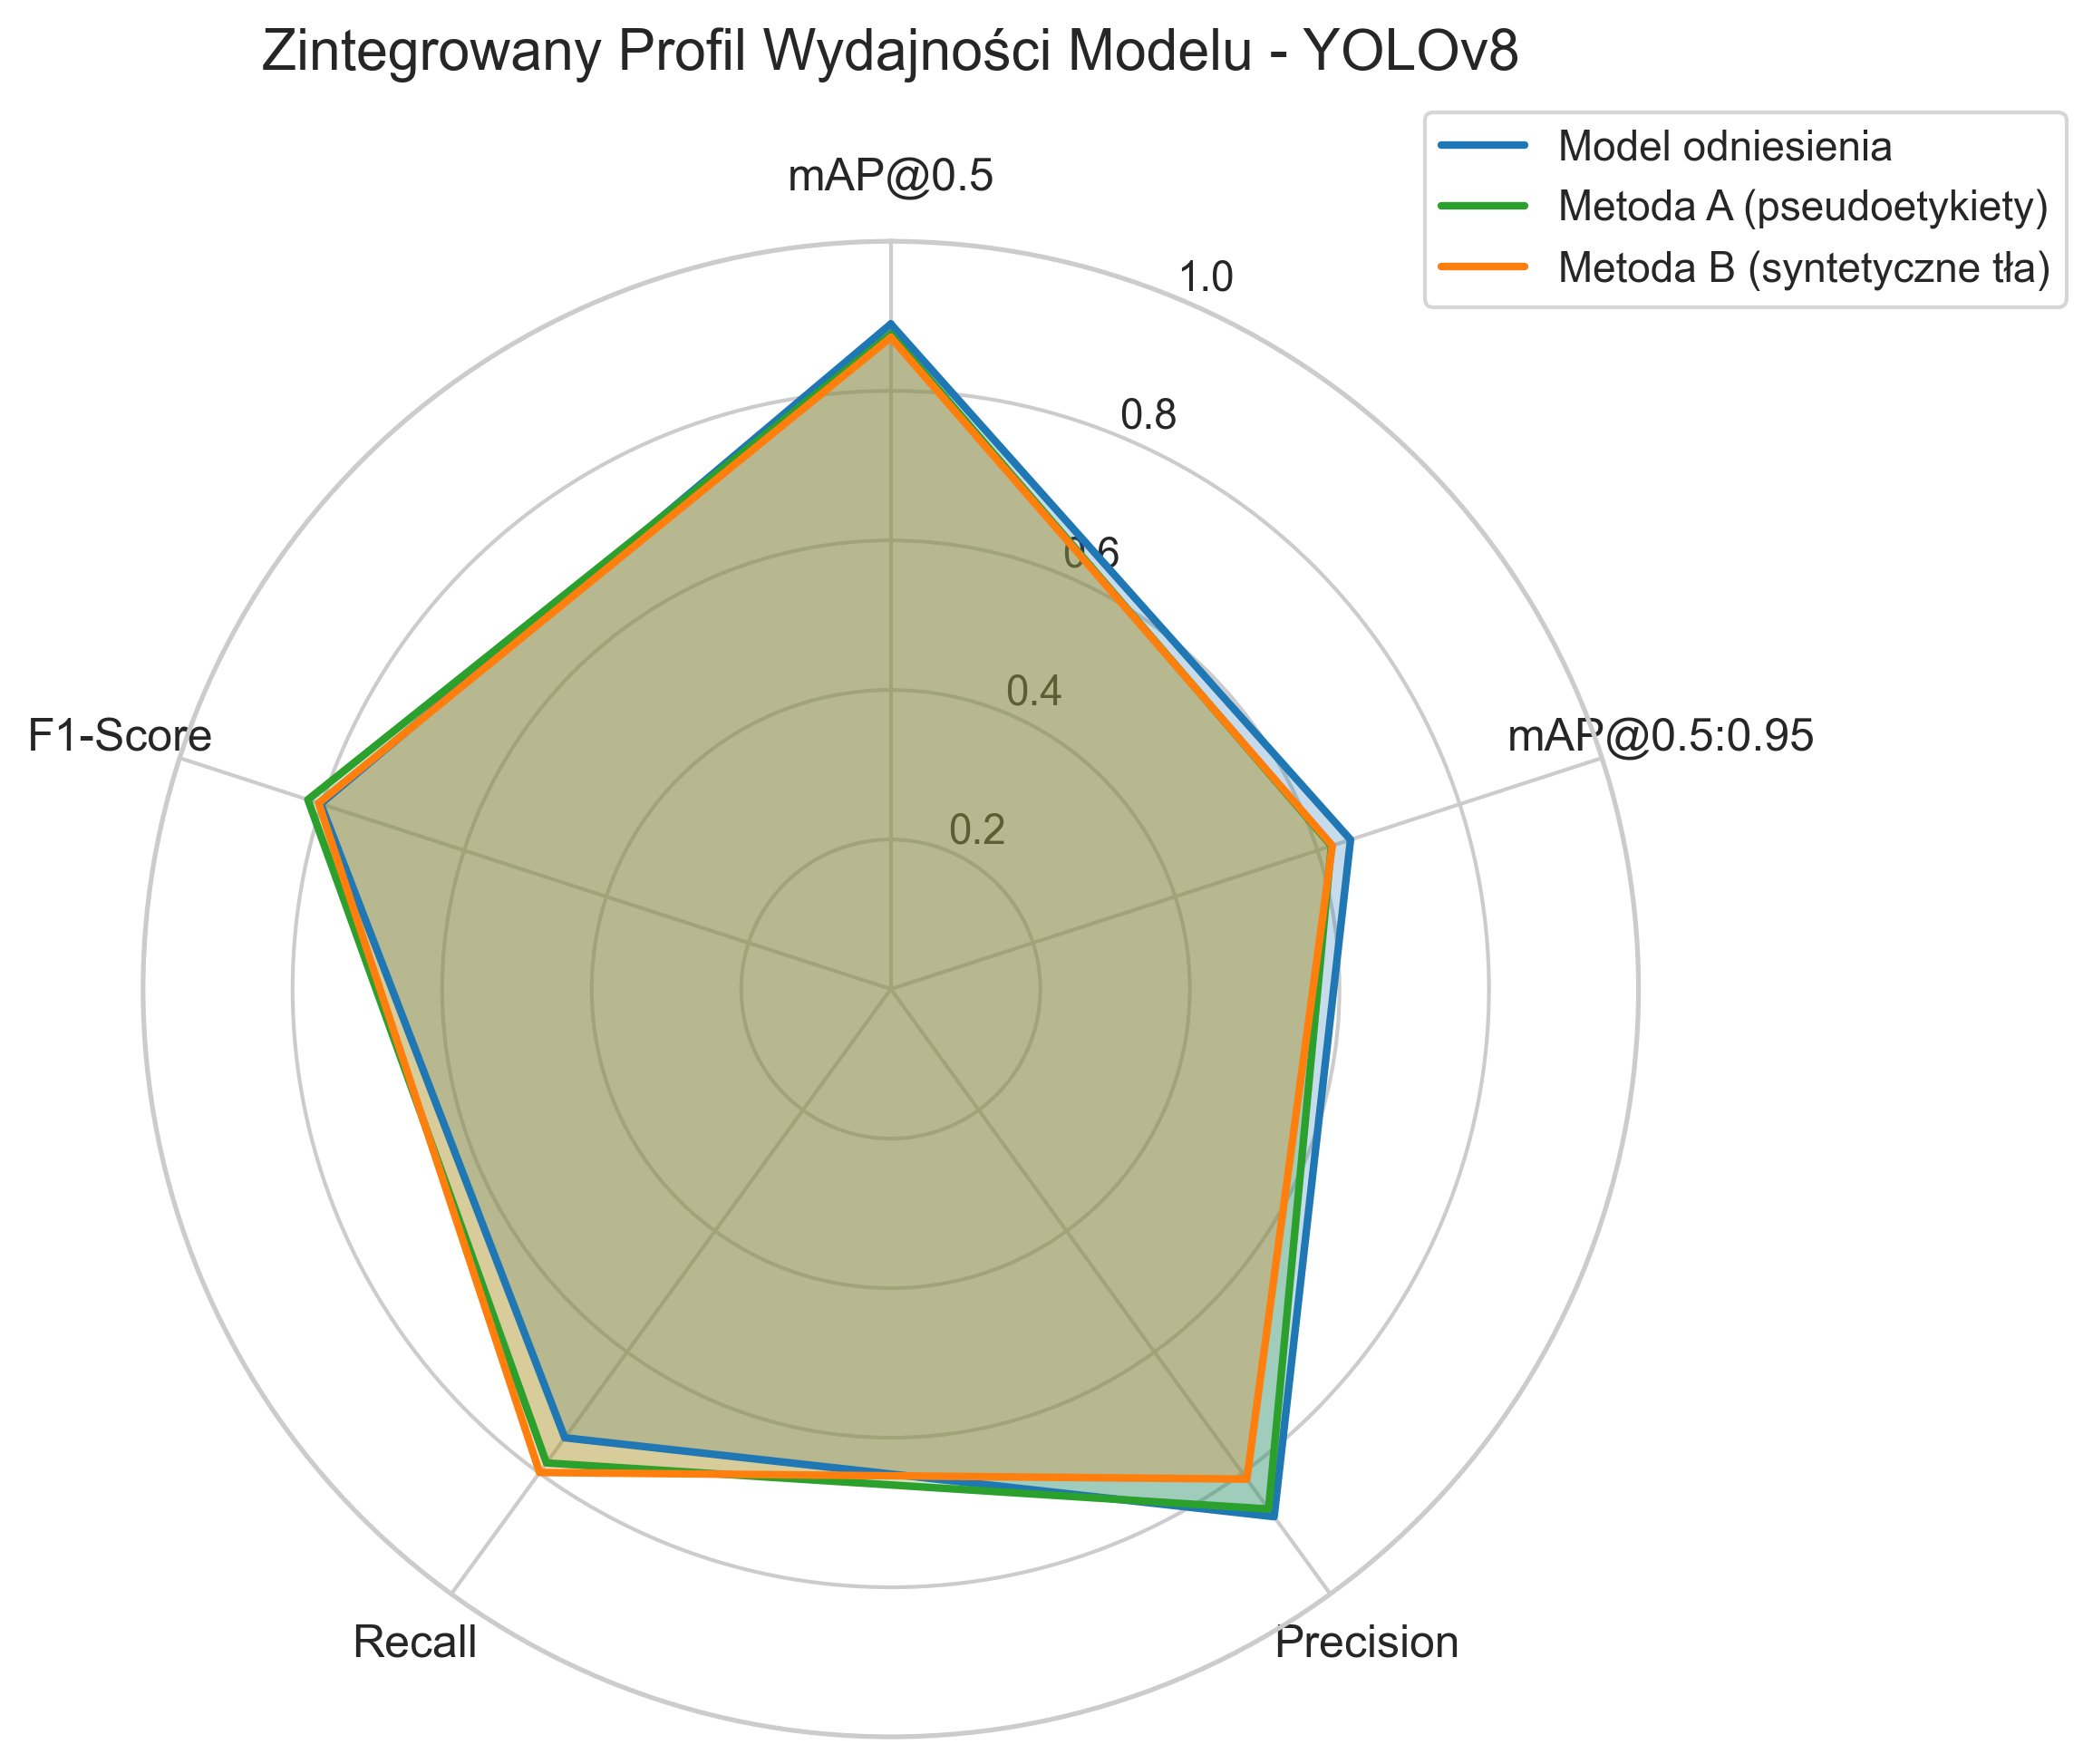
\includegraphics[width=0.8\linewidth]{Pics/Charts/wykres_5_radar_YOLOv8.png}
\caption{Zintegrowany profil wydajności modelu YOLOv8n na zbiorze walidacyjnym.}
\label{fig:radar_yolo8}
\end{figure}

\begin{figure}[htbp]
\centering
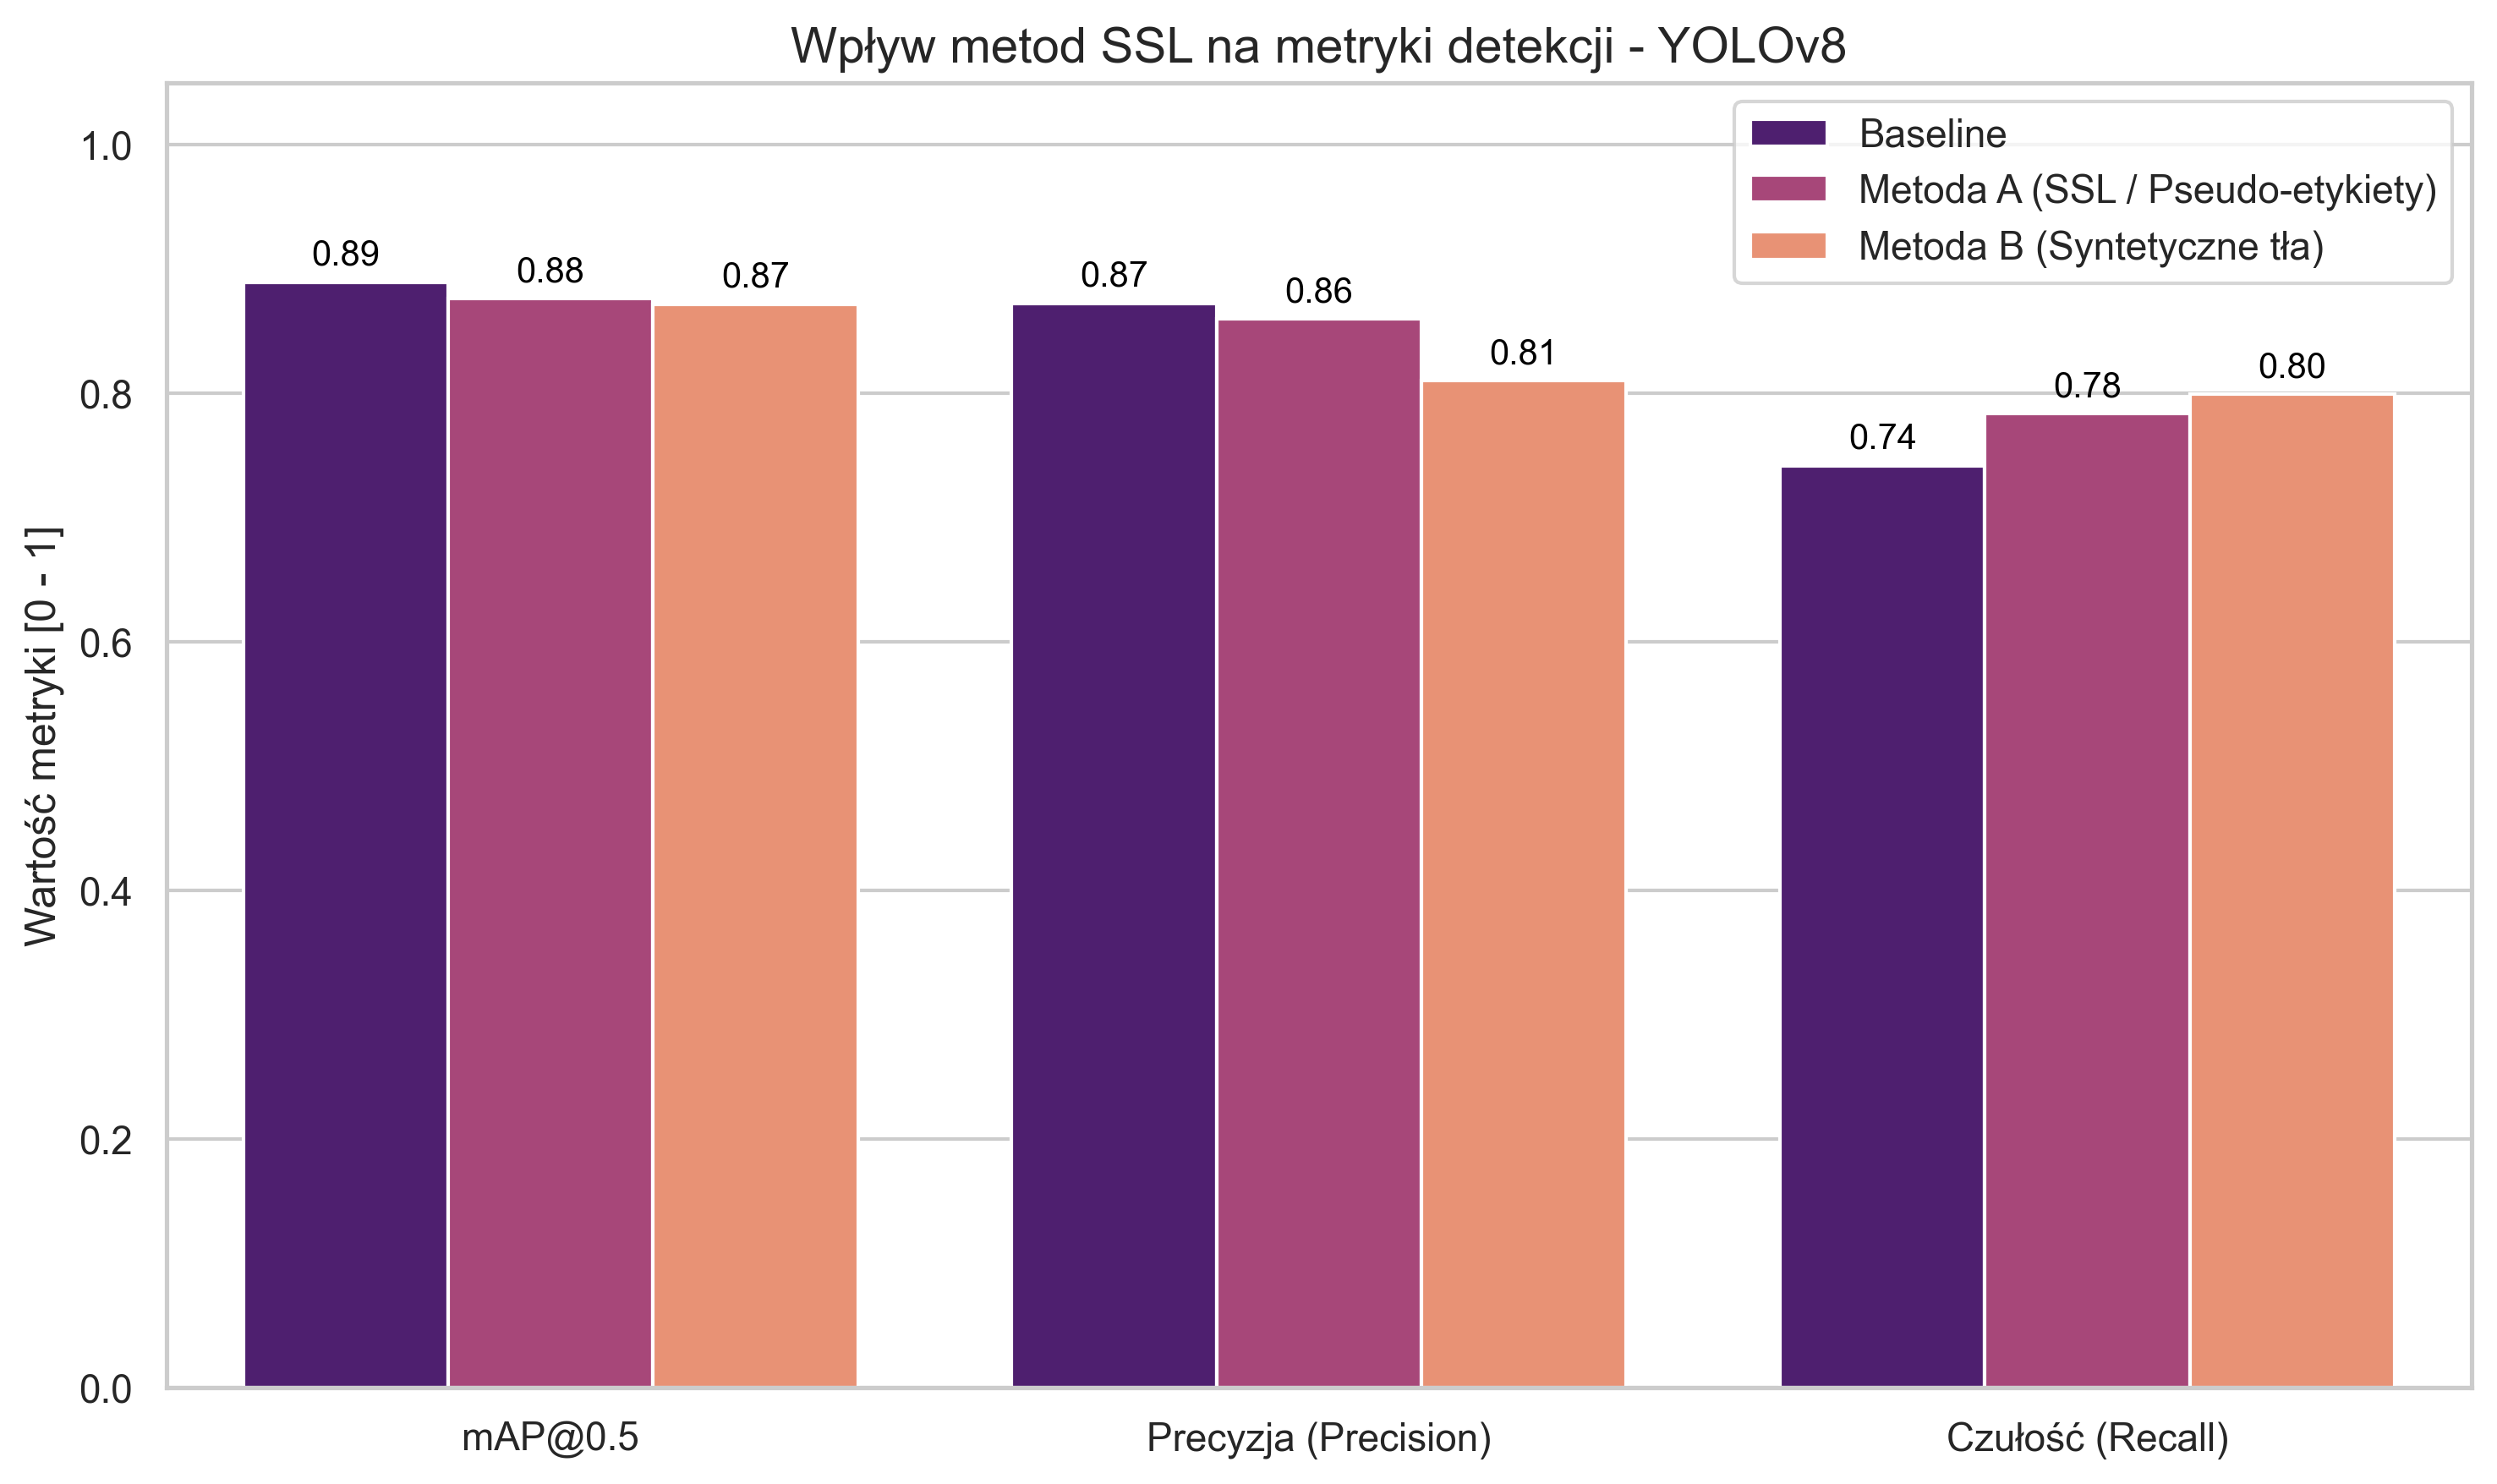
\includegraphics[width=0.8\linewidth]{Pics/Charts/wykres_1_metryki_YOLOv8.png}
\caption{Wpływ metod SSL na metryki detekcji modelu YOLOv8n na zbiorze walidacyjnym.}
\label{fig:bars_yolo8}
\end{figure}

\begin{figure}[htbp]
\centering
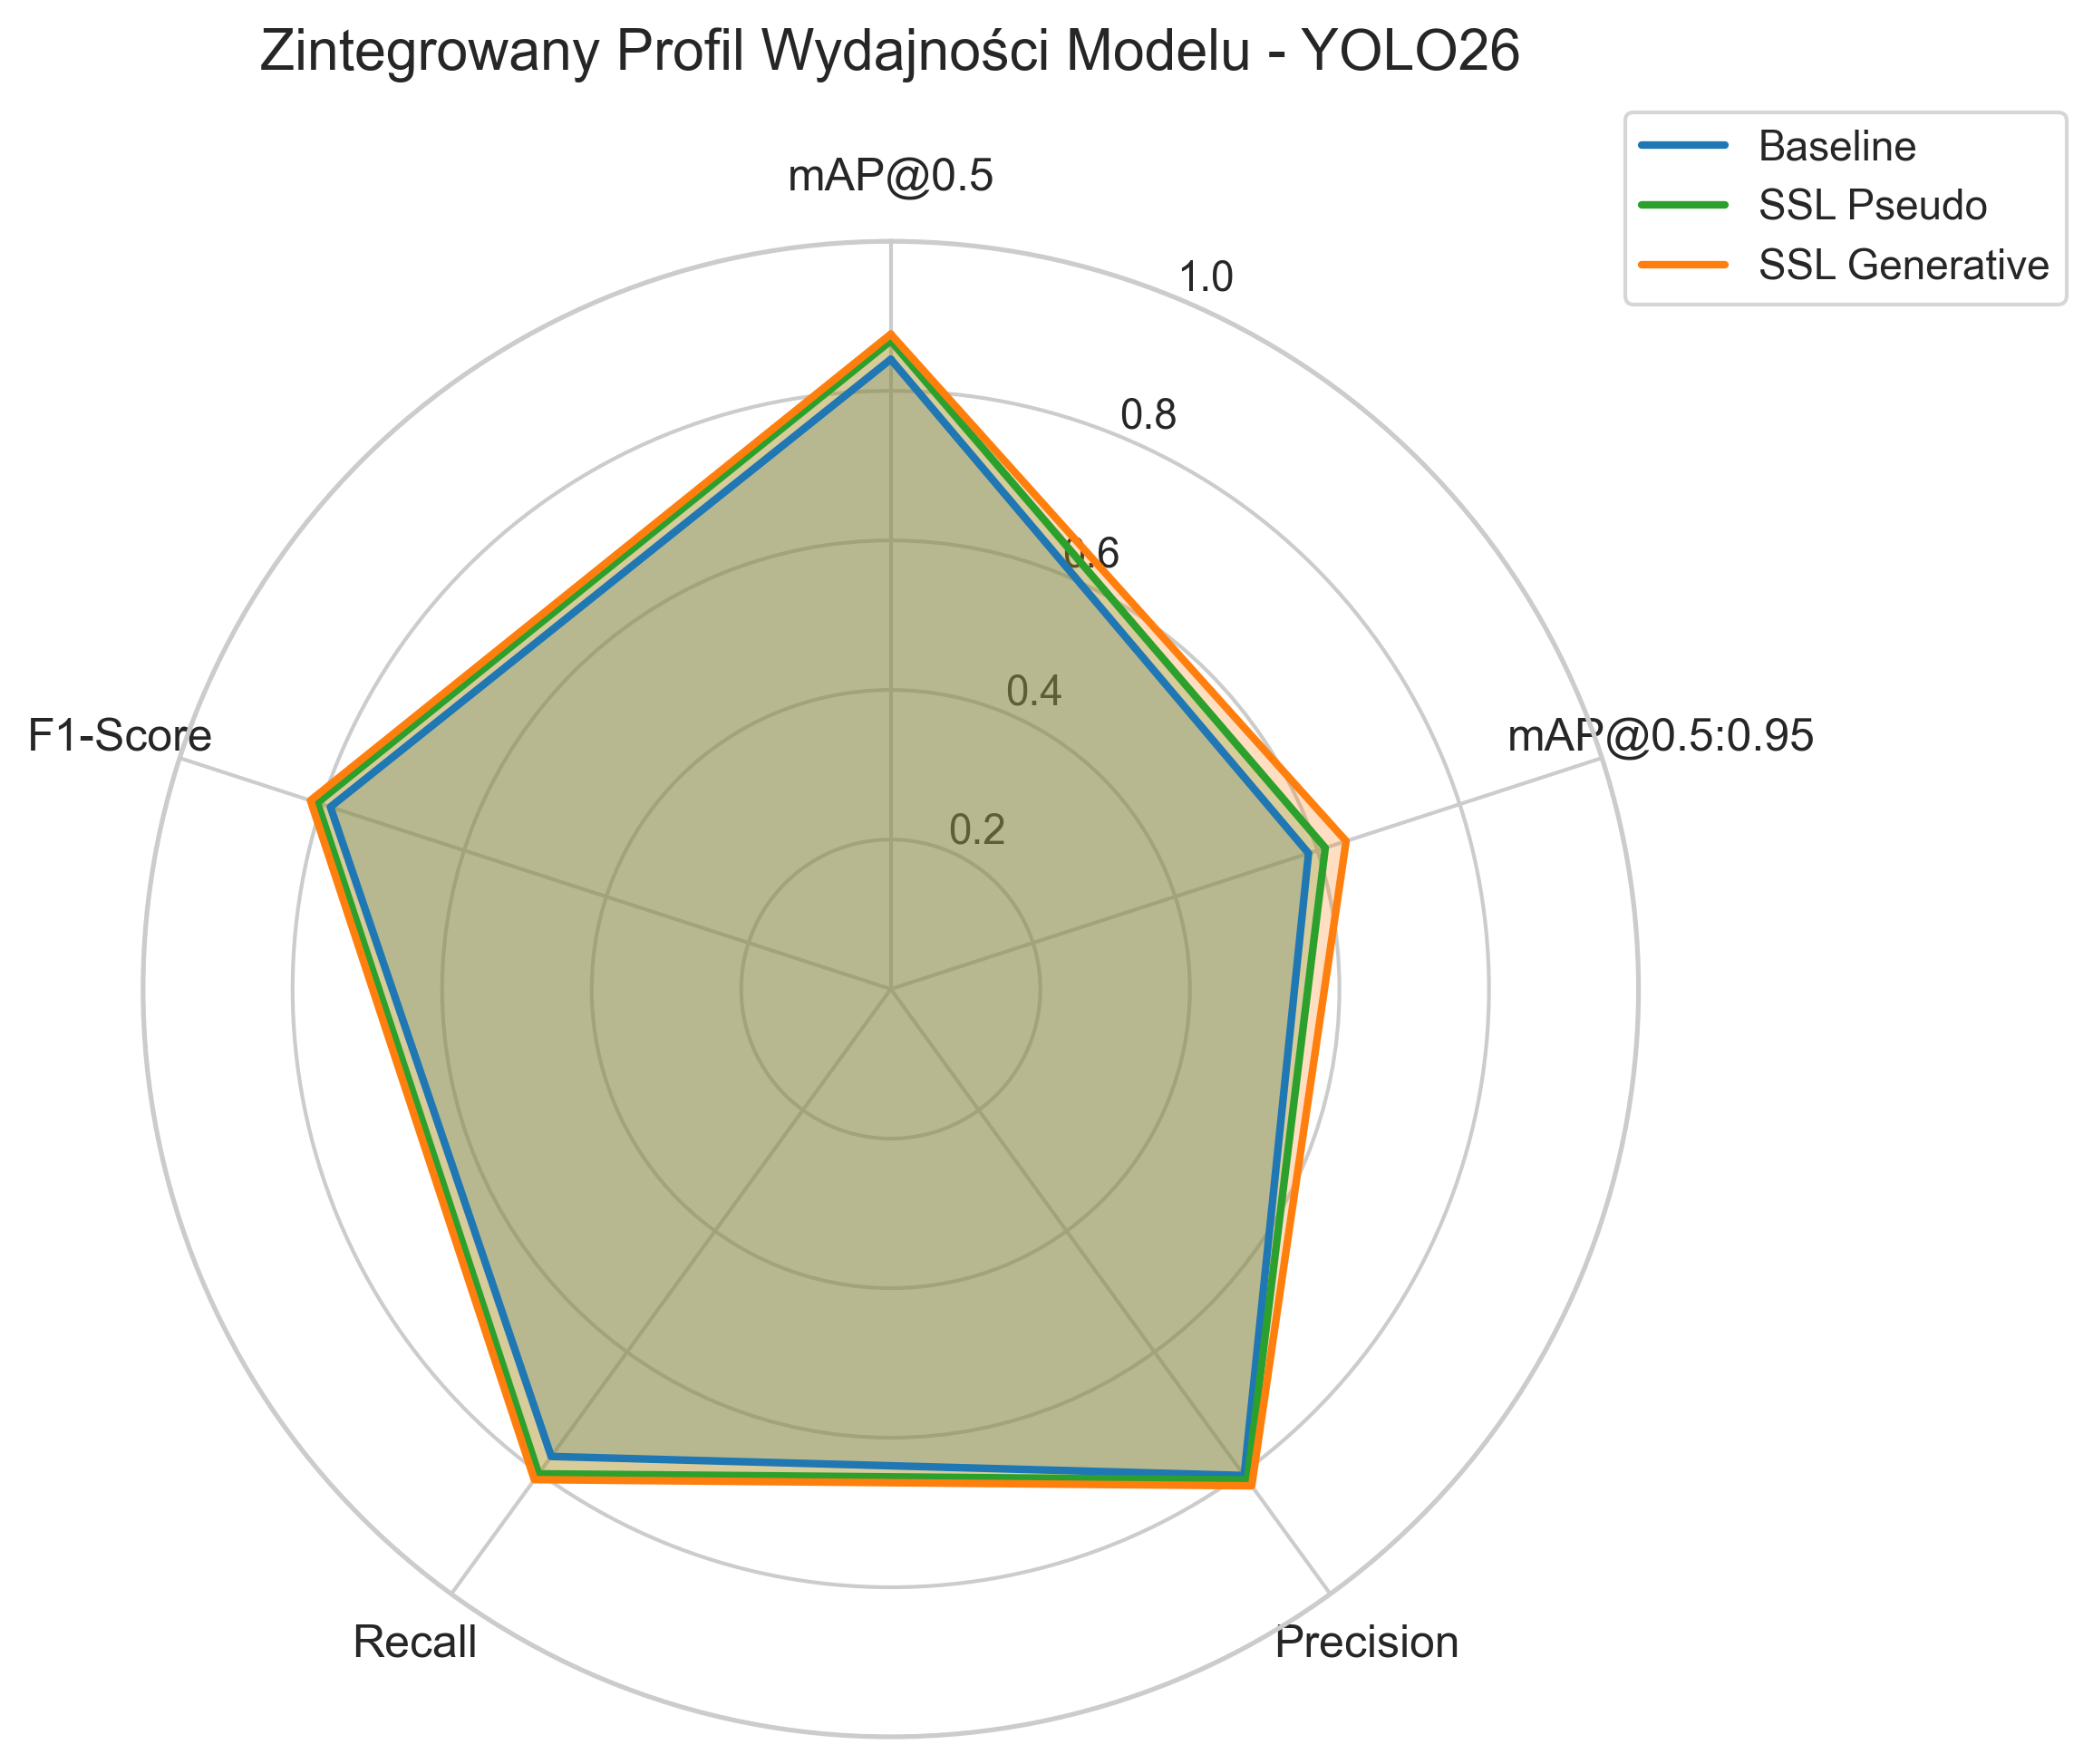
\includegraphics[width=0.8\linewidth]{Pics/Charts/wykres_5_radar_YOLO26.png}
\caption{Zintegrowany profil wydajności modelu YOLOv26n na zbiorze walidacyjnym.}
\label{fig:radar_yolo26}
\end{figure}

\begin{figure}[htbp]
\centering
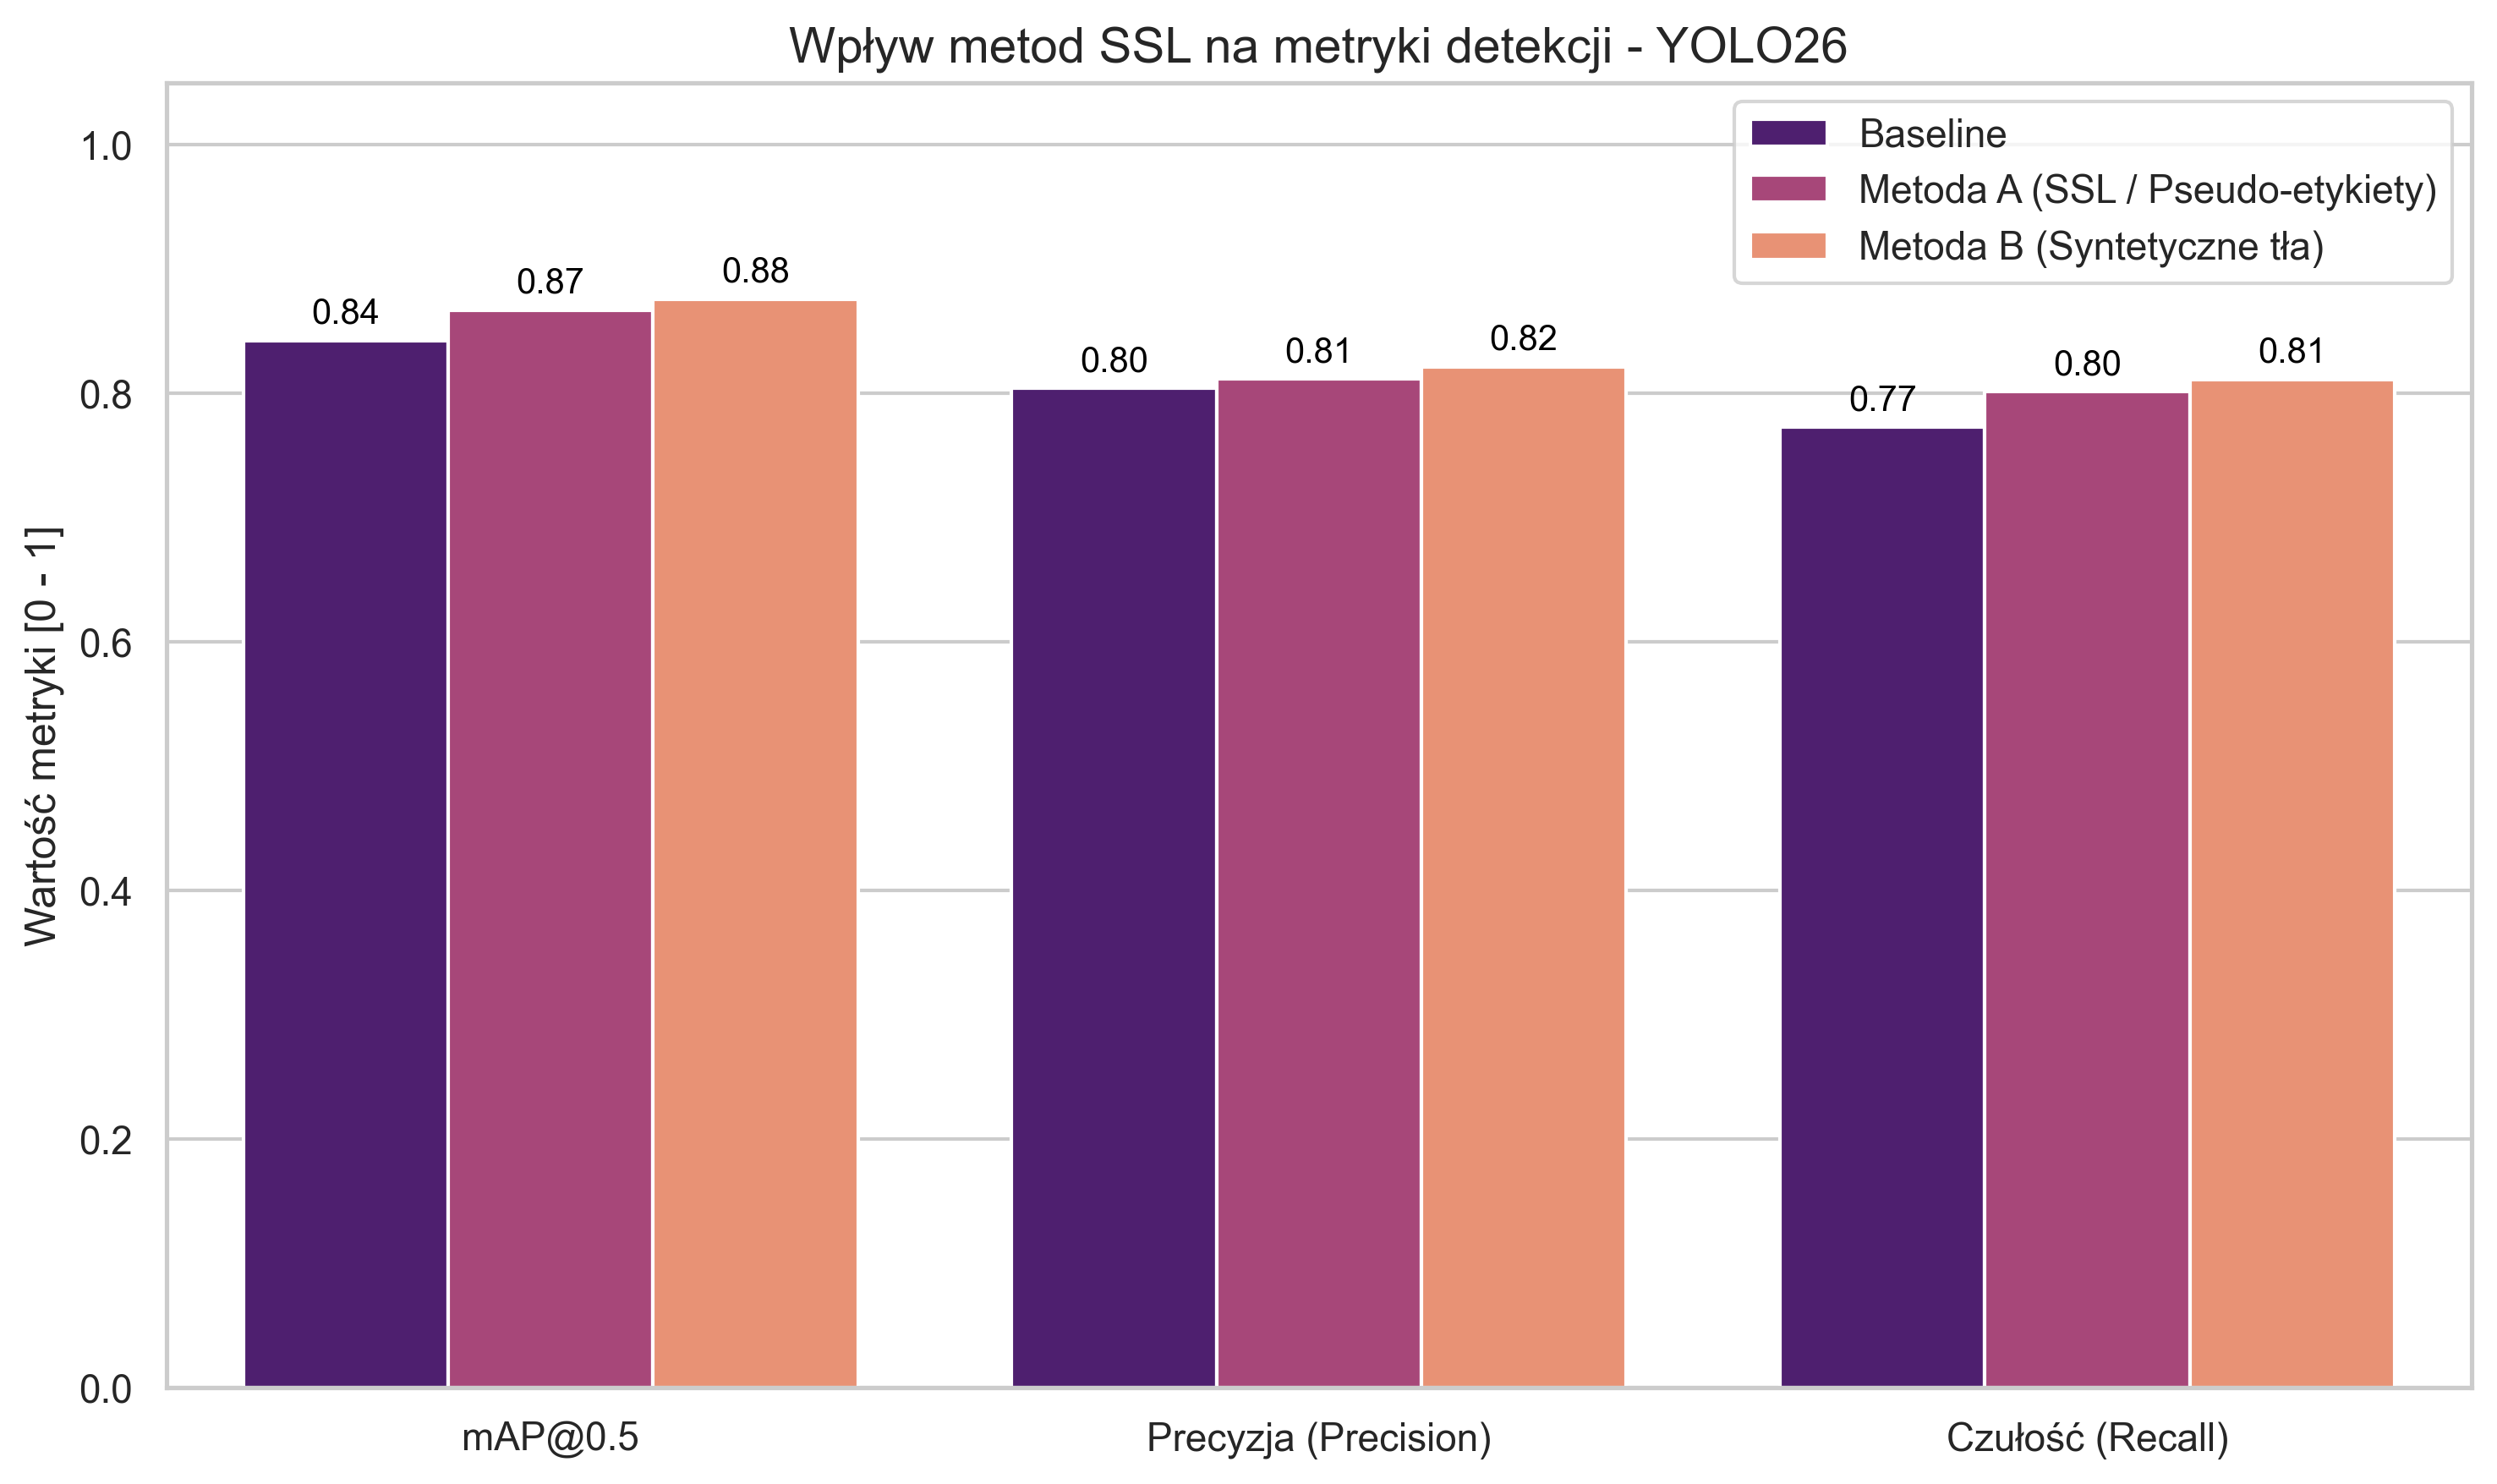
\includegraphics[width=0.8\linewidth]{Pics/Charts/wykres_1_metryki_YOLO26.png}
\caption{Wpływ metod SSL na metryki detekcji modelu YOLOv26n na zbiorze walidacyjnym.}
\label{fig:bars_yolo26}
\end{figure}

Z~kolei model YOLOv26n osiągnął nieco niższe wyniki referencyjne (mAP@0.5 równe 0.823, precyzja 0.807, czułość 0.737). Niższa czułość sugeruje, że model ten pomijał część obiektów docelowych, natomiast analiza fałszywych detekcji przedstawiona w~dalszej części rozdziału wskazuje, że wariant ten wymagał dodatkowej regularyzacji. Minimum funkcji straty walidacyjnej wystąpiło w~233. epoce (Rysunek \ref{fig:loss_yolo26}).

% MIEJSCE NA NOWE WYKRESY FUNKCJI STRATY (ANALIZA PRZEUCZENIA) DLA YOLO
\begin{figure}[htbp]
\centering
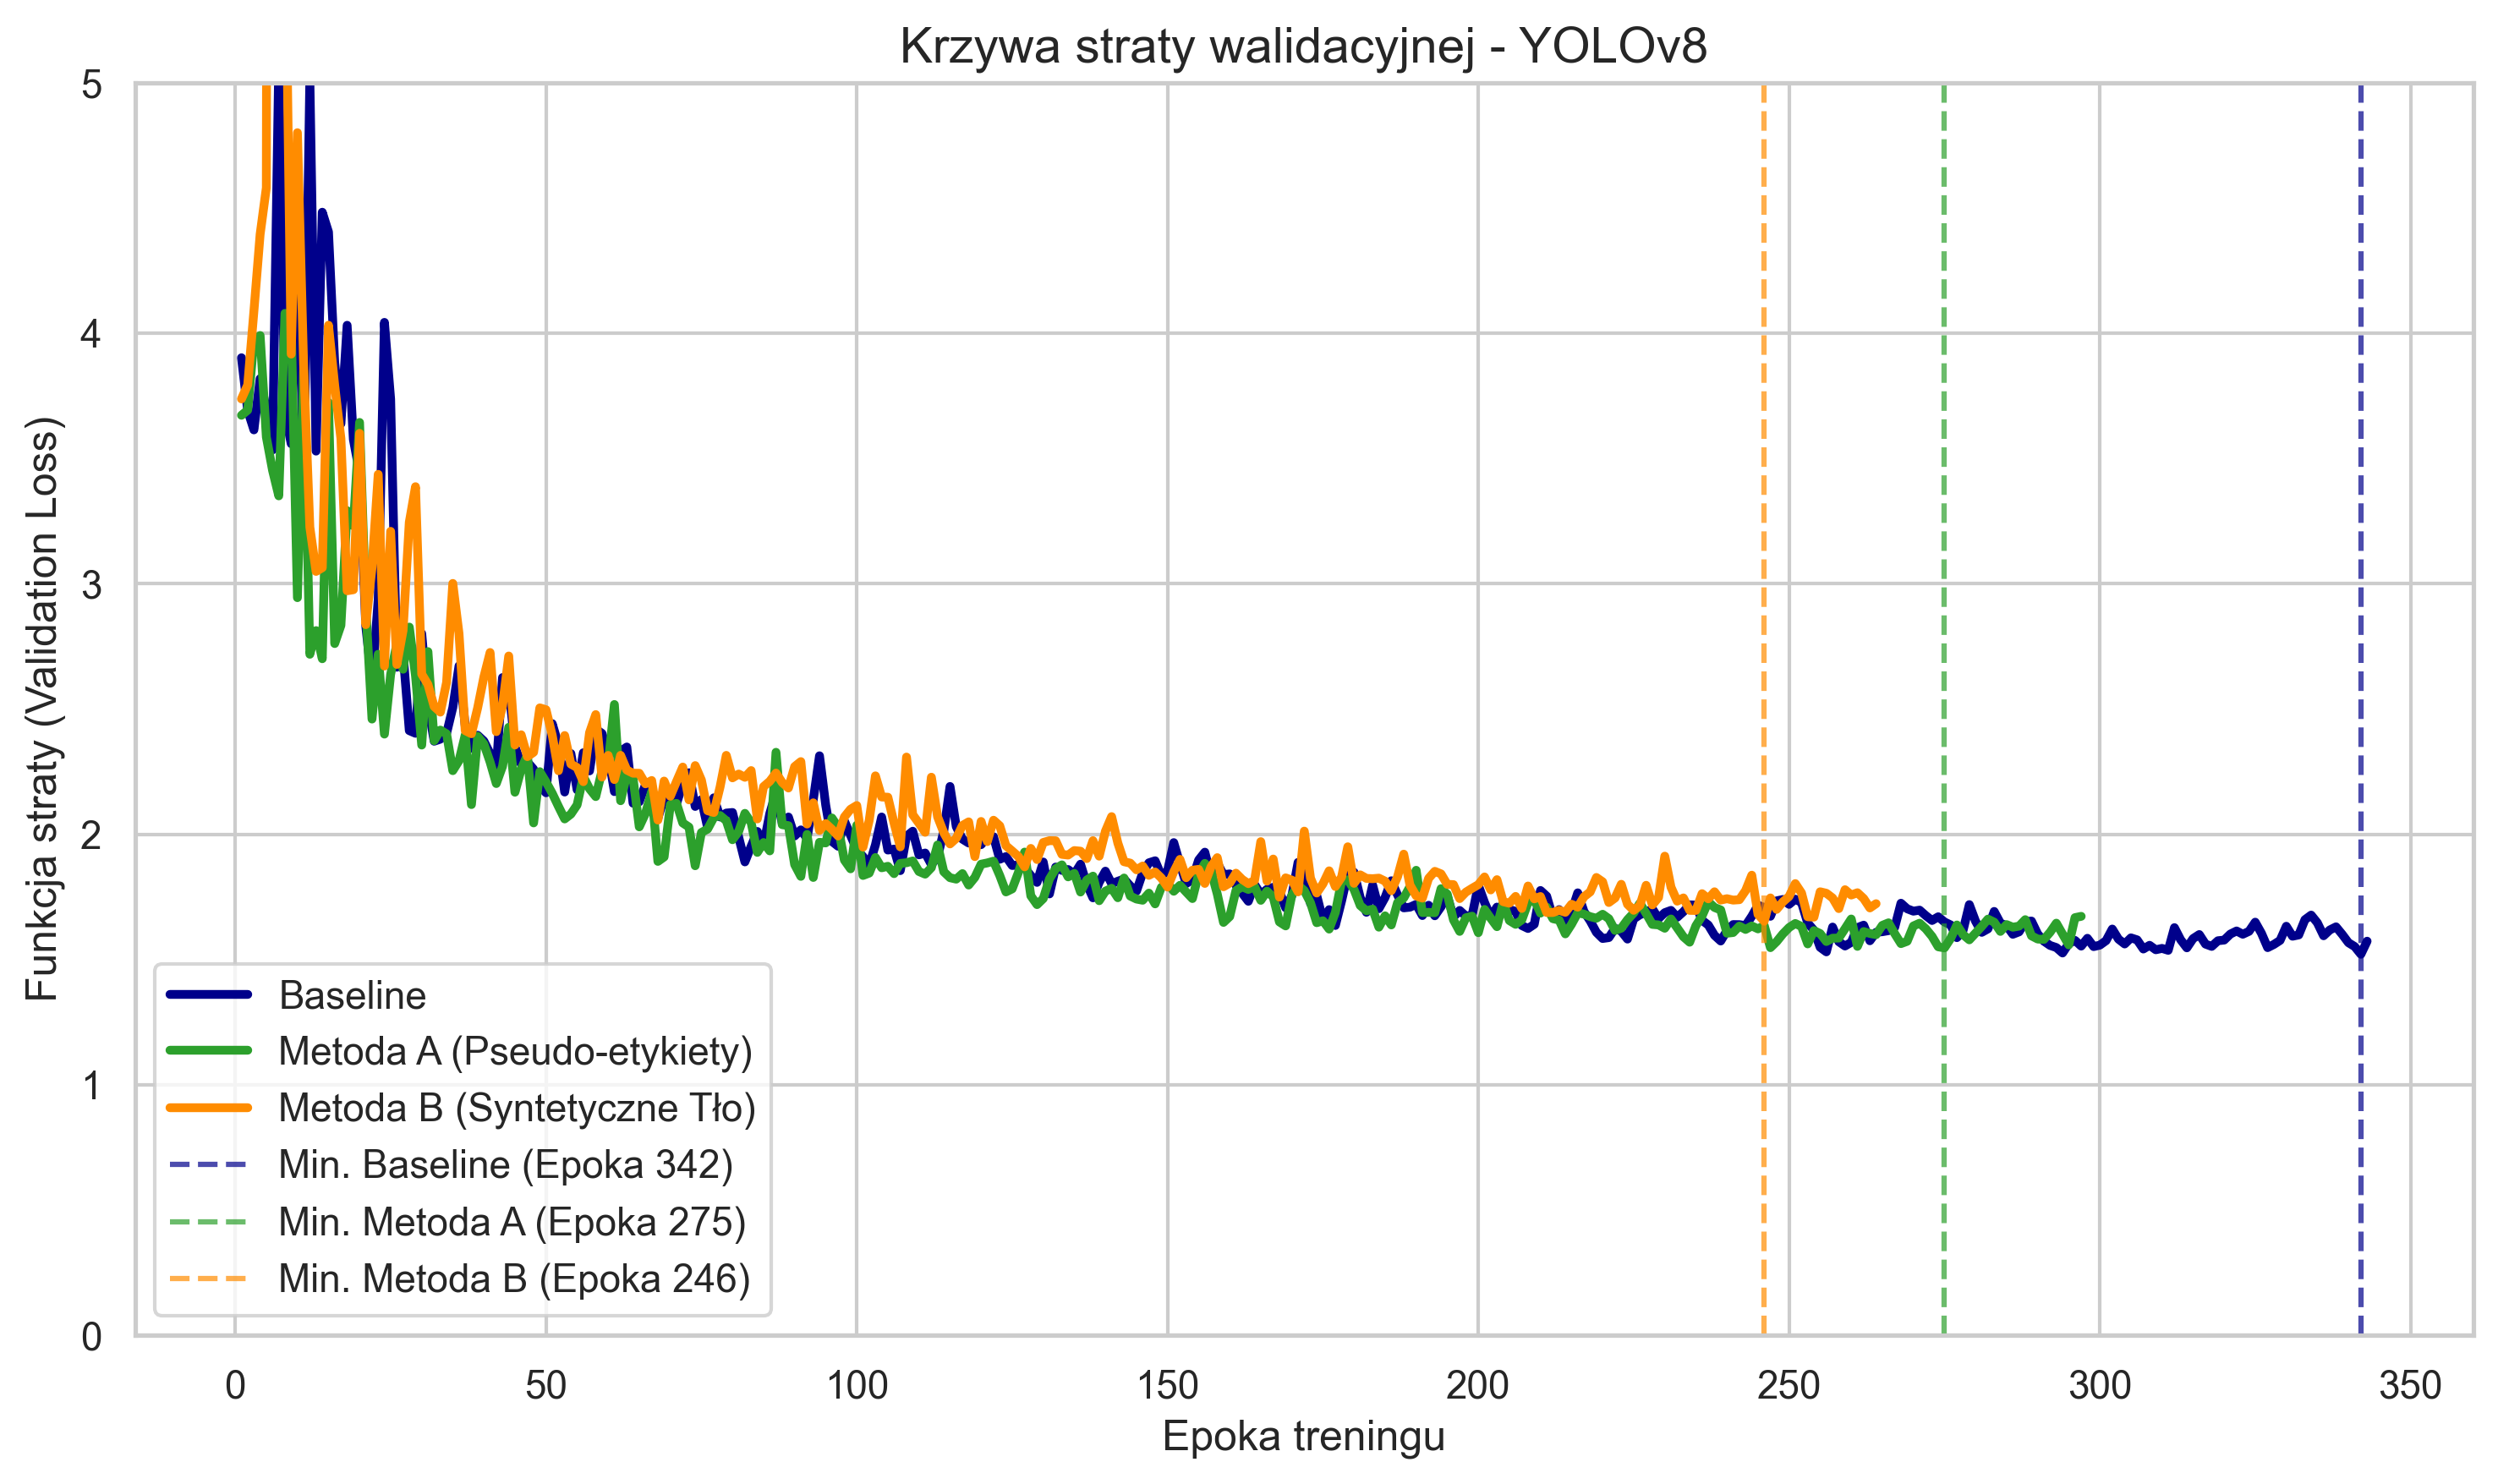
\includegraphics[width=1\linewidth]{Pics/Charts/wykres_2_loss_YOLOv8.png}
\caption{Krzywe straty dla danych ze zbioru walidacyjnego -- YOLOv8n.}
\label{fig:loss_yolo8}
\end{figure}

\begin{figure}[htbp]
\centering
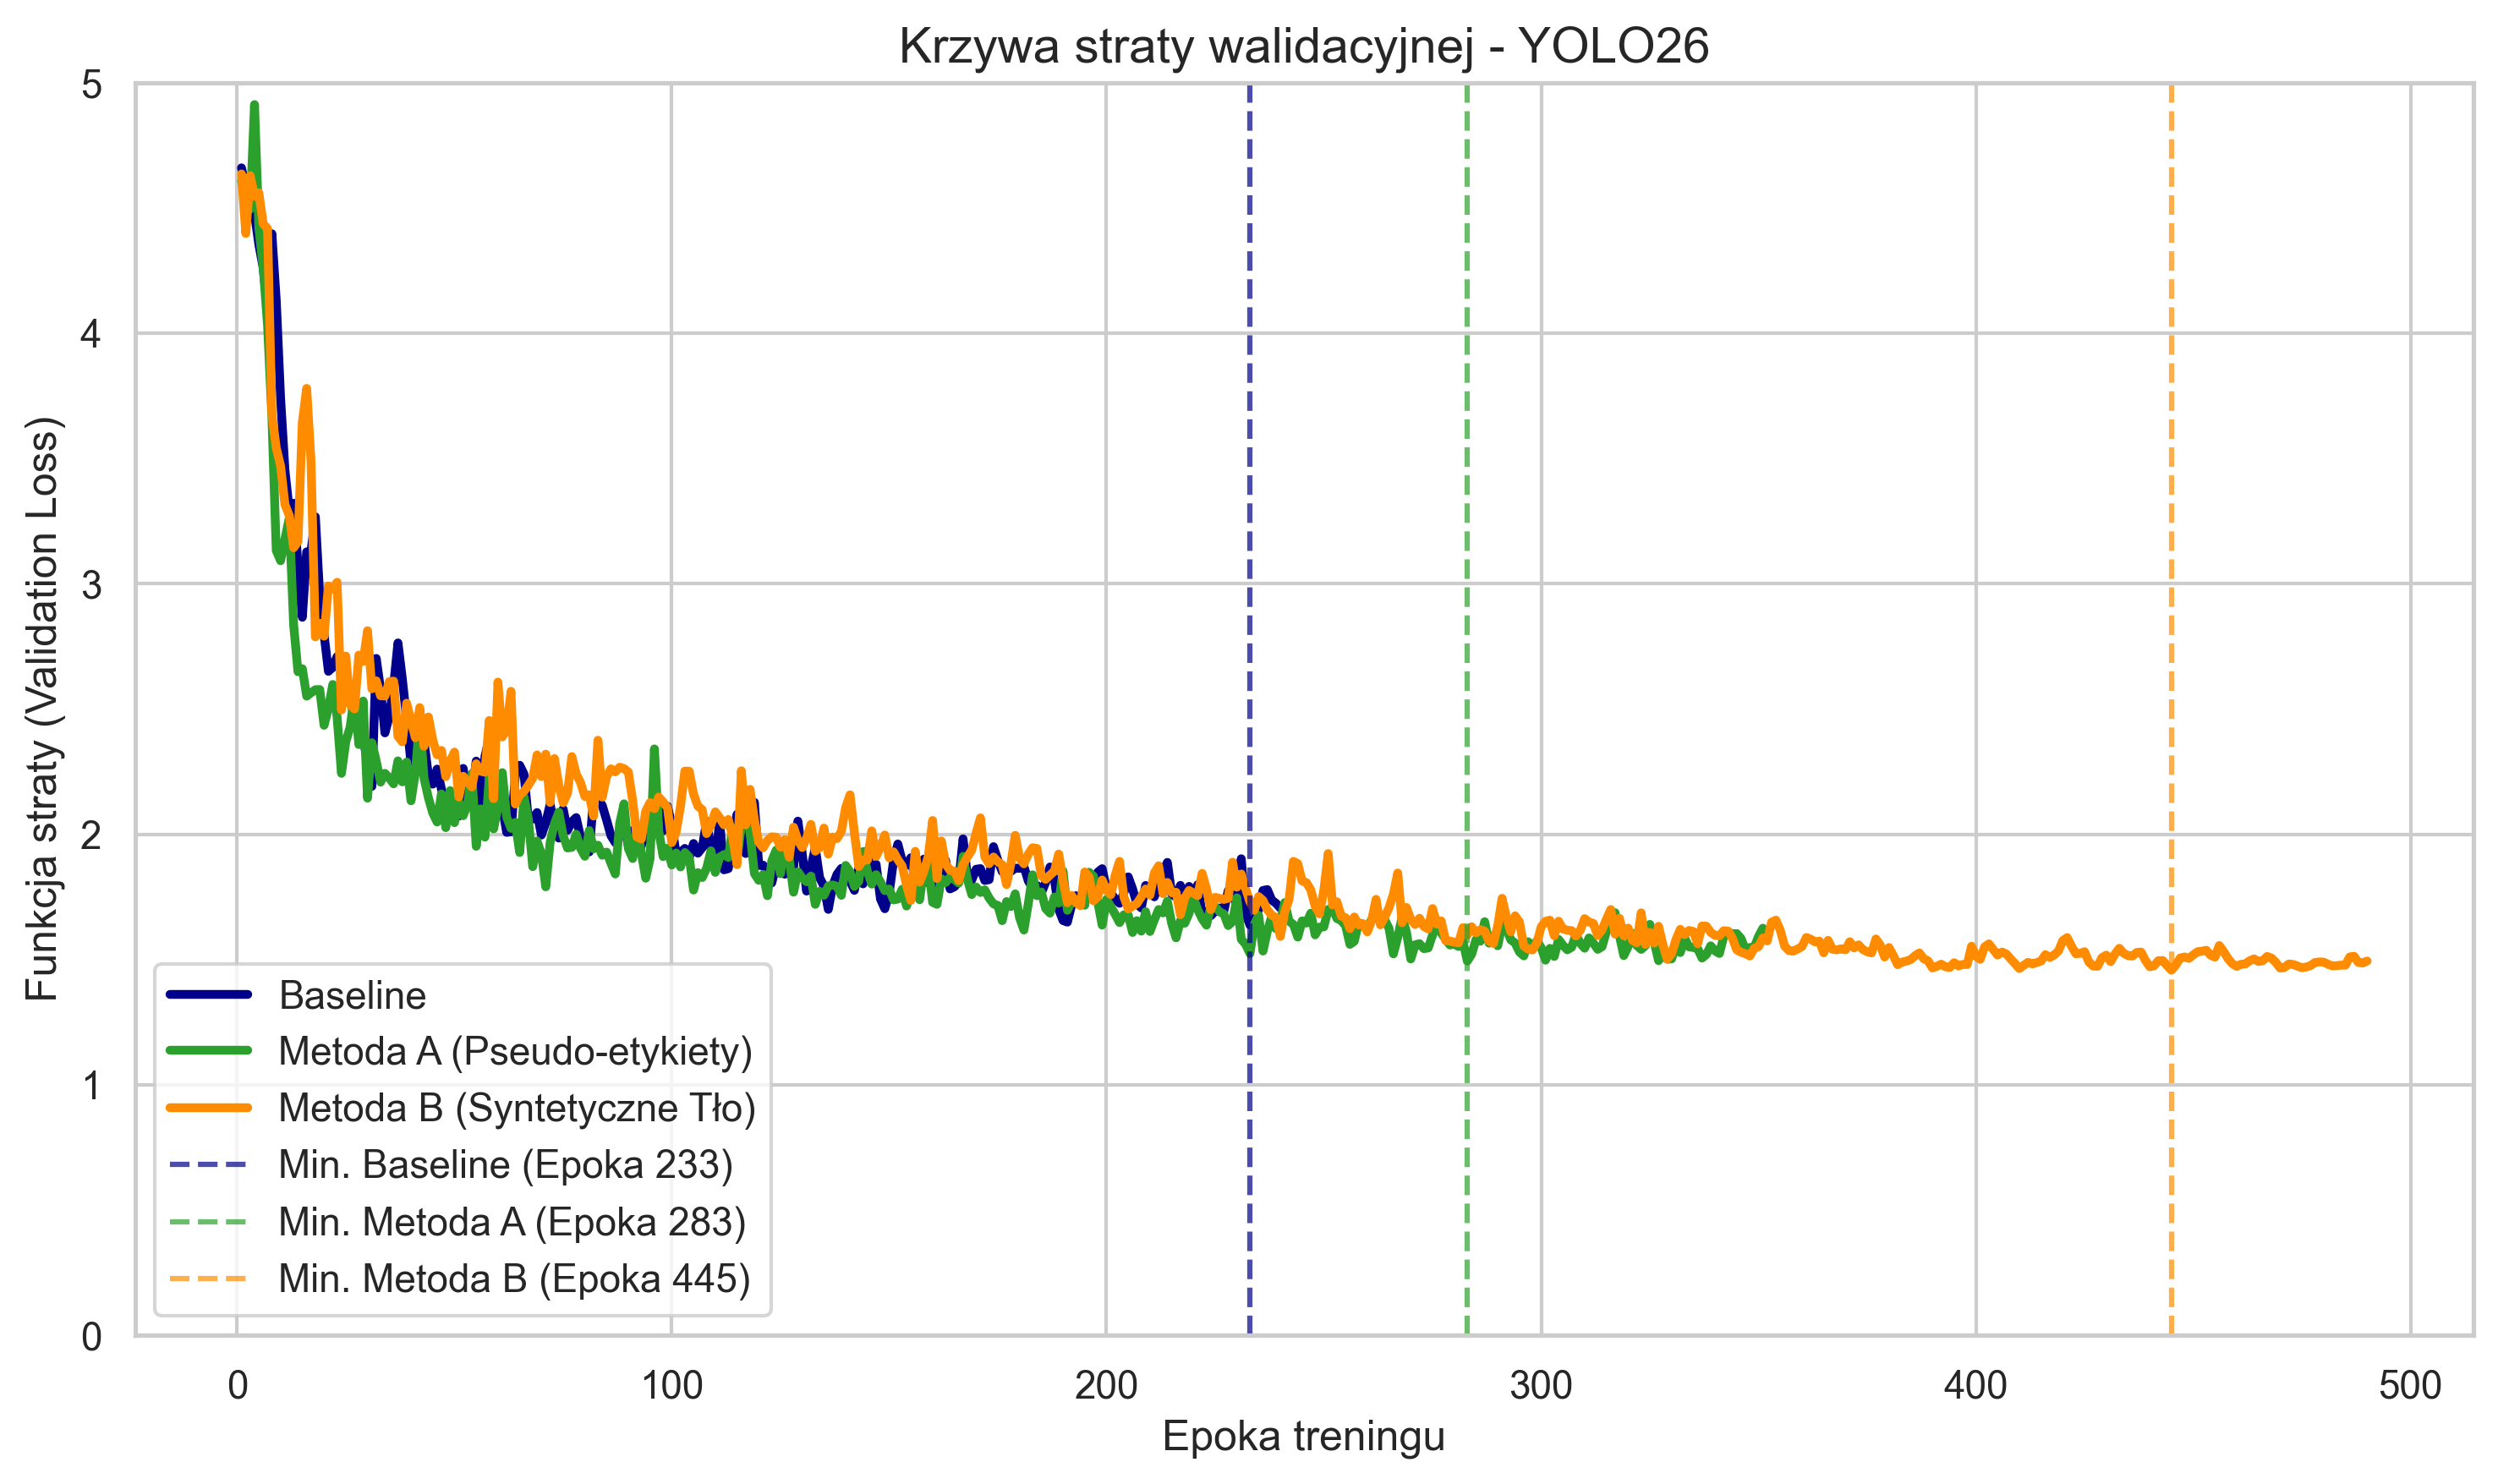
\includegraphics[width=1\linewidth]{Pics/Charts/wykres_2_loss_YOLO26.png}
\caption{Krzywe straty dla danych ze zbioru walidacyjnego -- YOLOv26n.}
\label{fig:loss_yolo26}
\end{figure}

\subsection{Wyniki dla architektury RT-DETR-L}

Analogicznemu procesowi ewaluacji poddano model RT-DETR-L. Jako że jest to architektura oparta na transformerach wizyjnych, weryfikacji podlegała jej dynamika zbieżności w~reżimie ograniczonej liczby danych.

Wyniki referencyjne metryk dla RT-DETR-L (Rysunek \ref{fig:radar_rtdetr} i~\ref{fig:bars_rtdetr}) były porównywalne z~wynikami YOLOv8n (mAP@0.5 równe 0.877, precyzja 0.829, czułość 0.817). Model dobrze radził sobie z~lokalizacją obiektów, jednak krzywa straty walidacyjnej (Rysunek \ref{fig:loss_rtdetr}) wskazuje na większą niestabilność procesu uczenia niż w~przypadku detektorów splotowych. Minimum straty walidacyjnej przypadło na 230. epokę.

% MIEJSCE NA WYKRESY DLA RT-DETR
\begin{figure}[htbp]
\centering
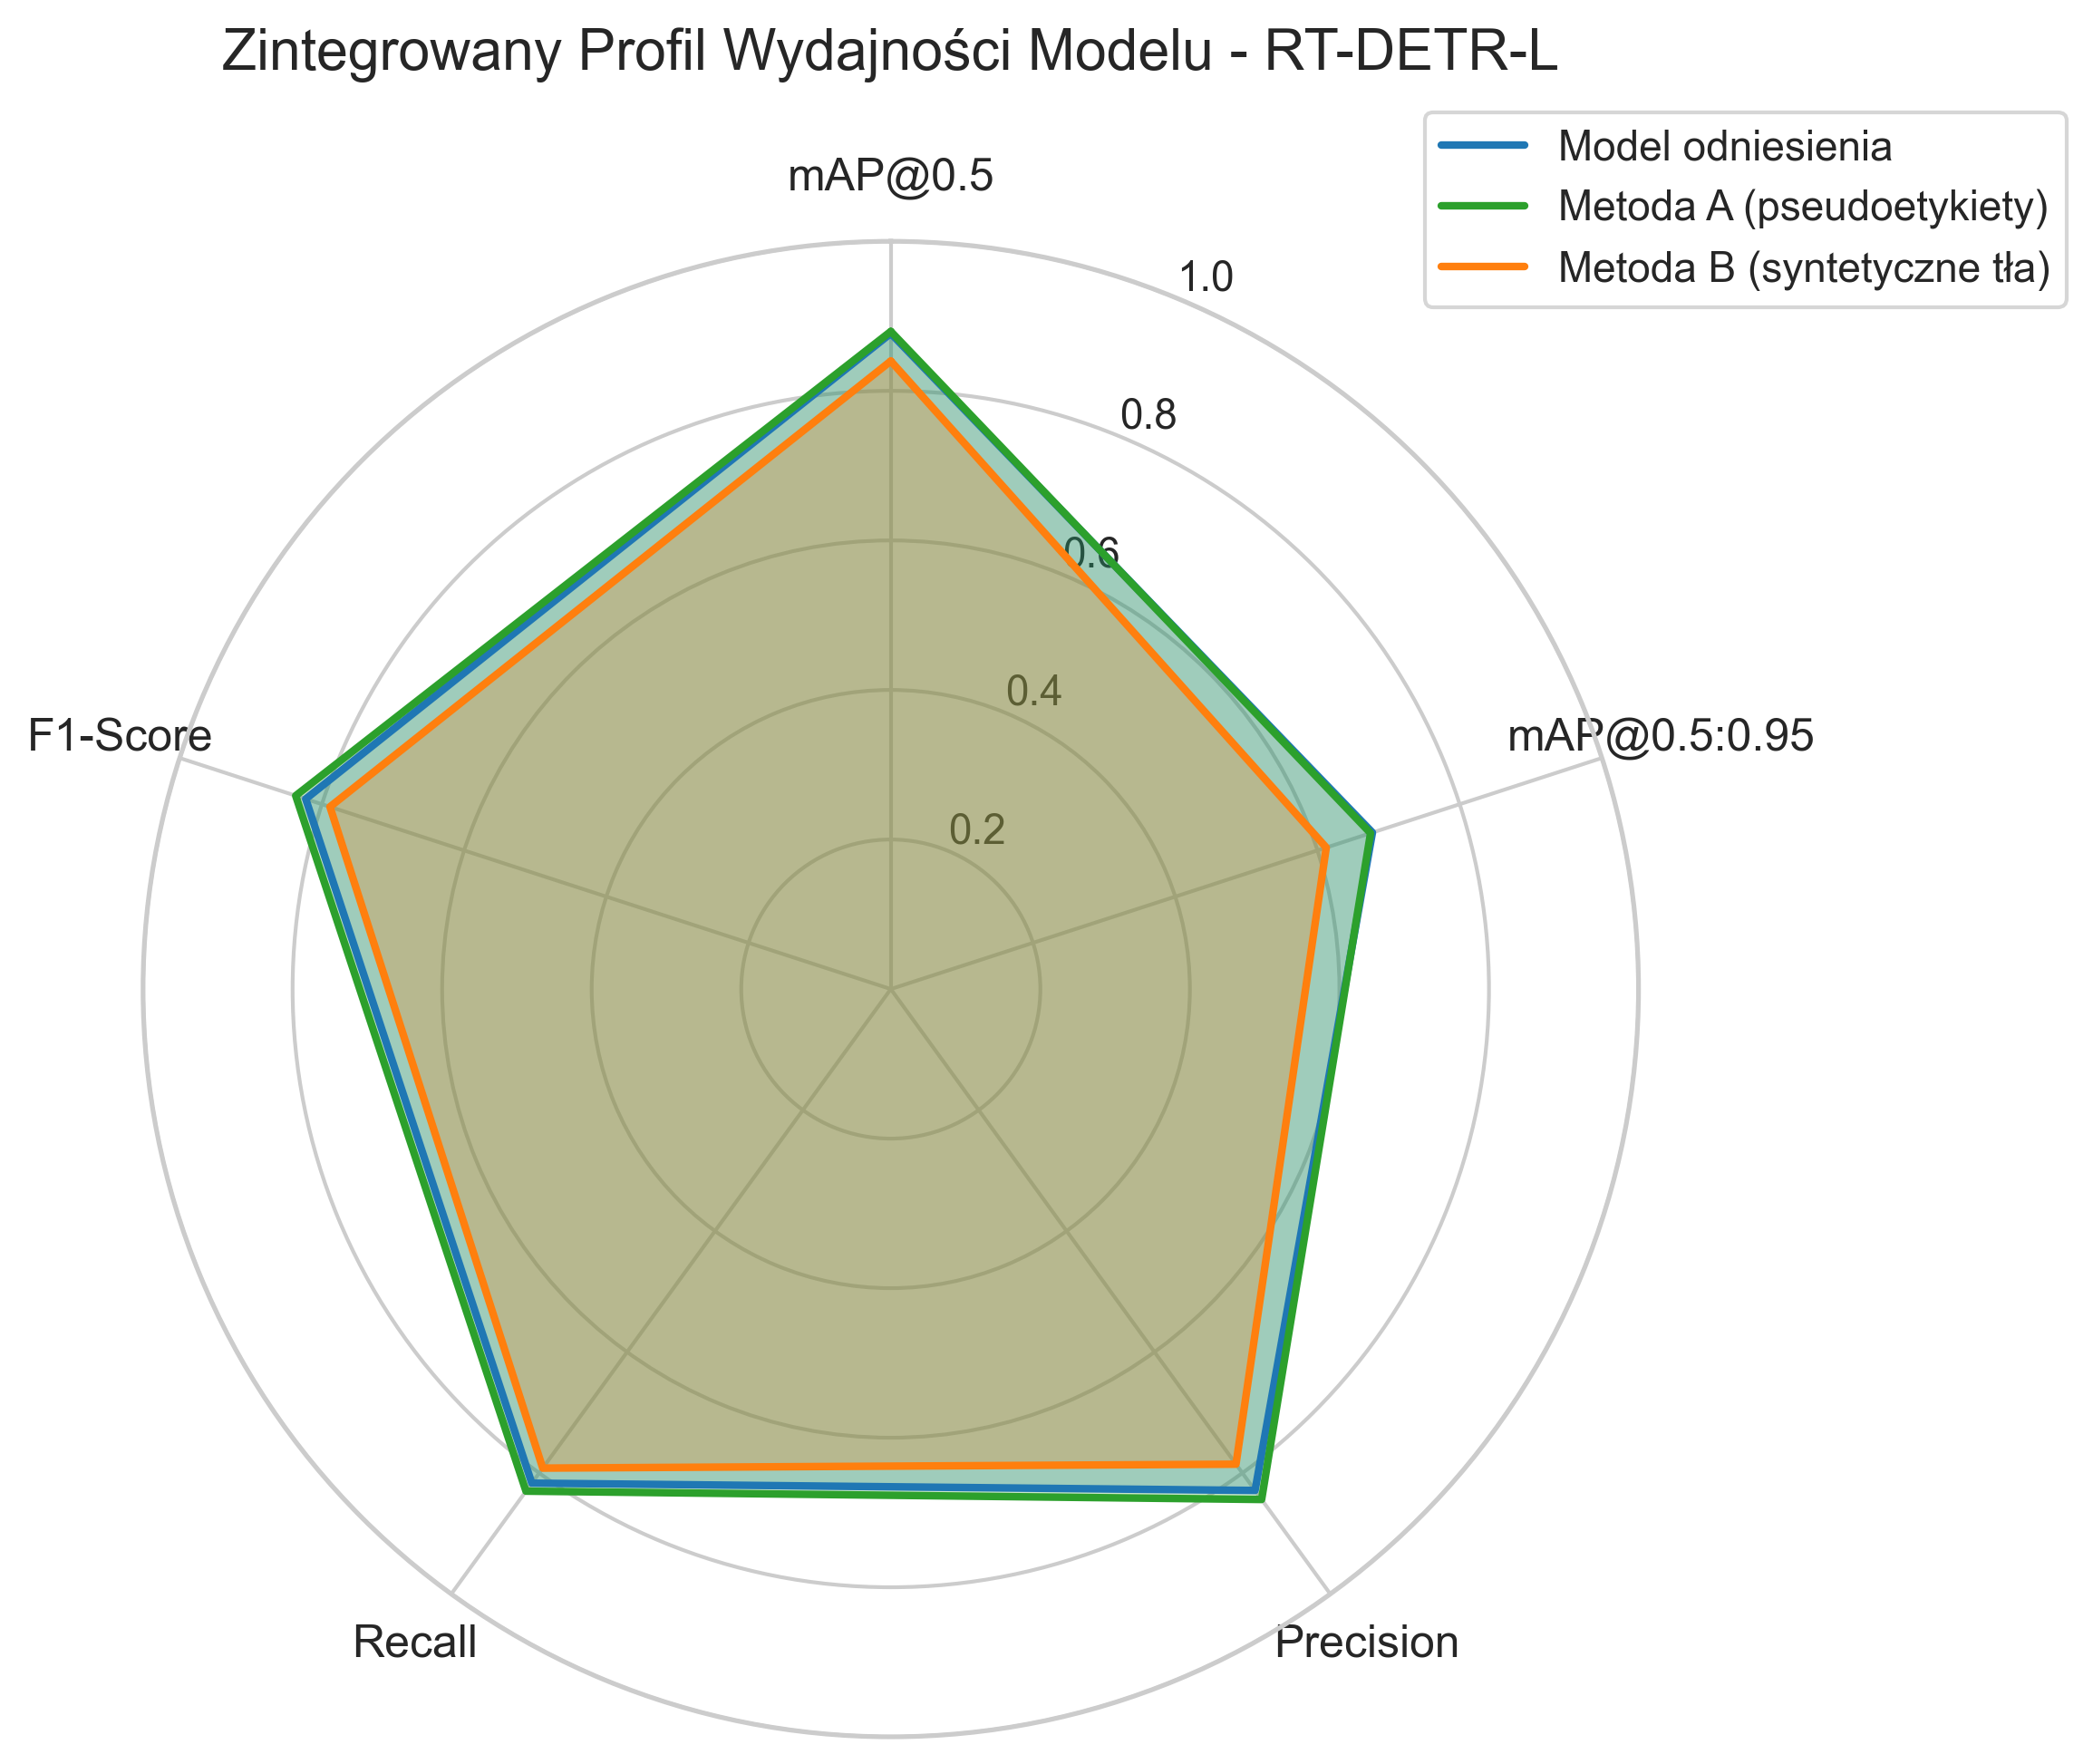
\includegraphics[width=0.8\linewidth]{Pics/Charts/wykres_5_radar_RT-DETR-L.png}
\caption{Zintegrowany profil wydajności modelu RT-DETR-L na zbiorze walidacyjnym.}
\label{fig:radar_rtdetr}
\end{figure}

\begin{figure}[htbp]
\centering
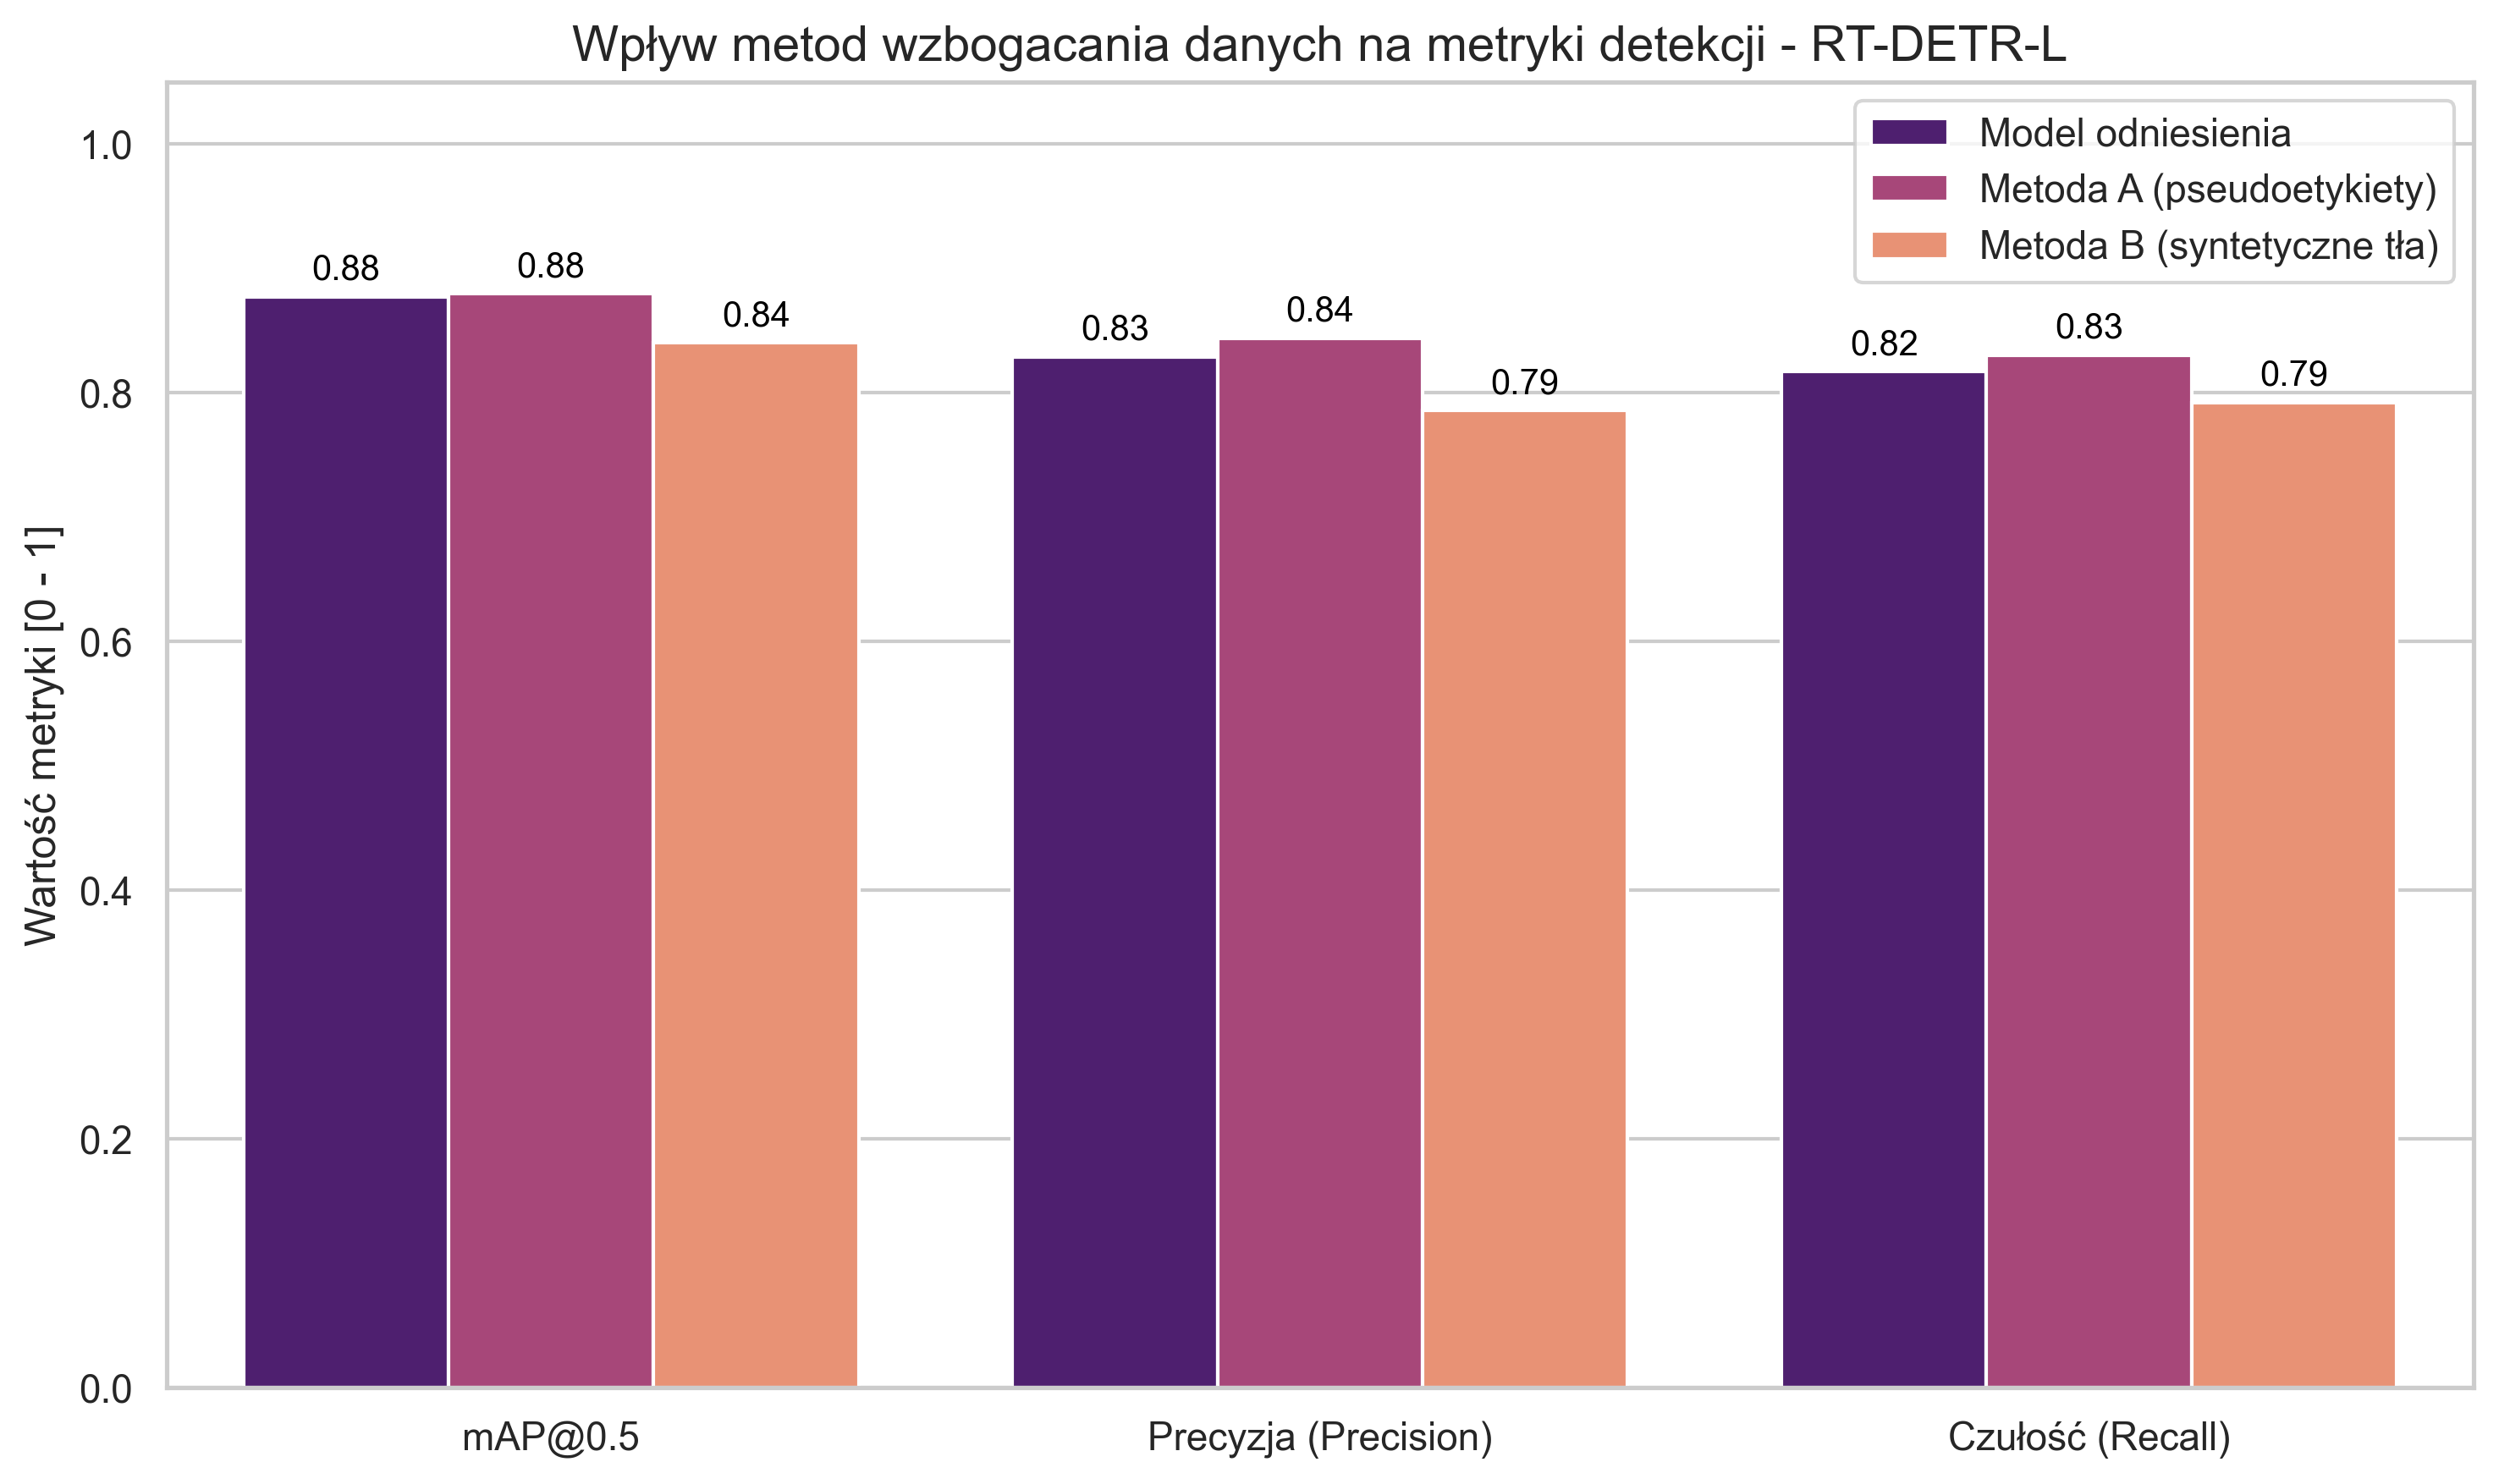
\includegraphics[width=0.8\linewidth]{Pics/Charts/wykres_1_metryki_RT-DETR-L.png}
\caption{Wpływ metod SSL na metryki detekcji modelu RT-DETR-L na zbiorze walidacyjnym.}
\label{fig:bars_rtdetr}
\end{figure}

\begin{figure}[htbp]
\centering
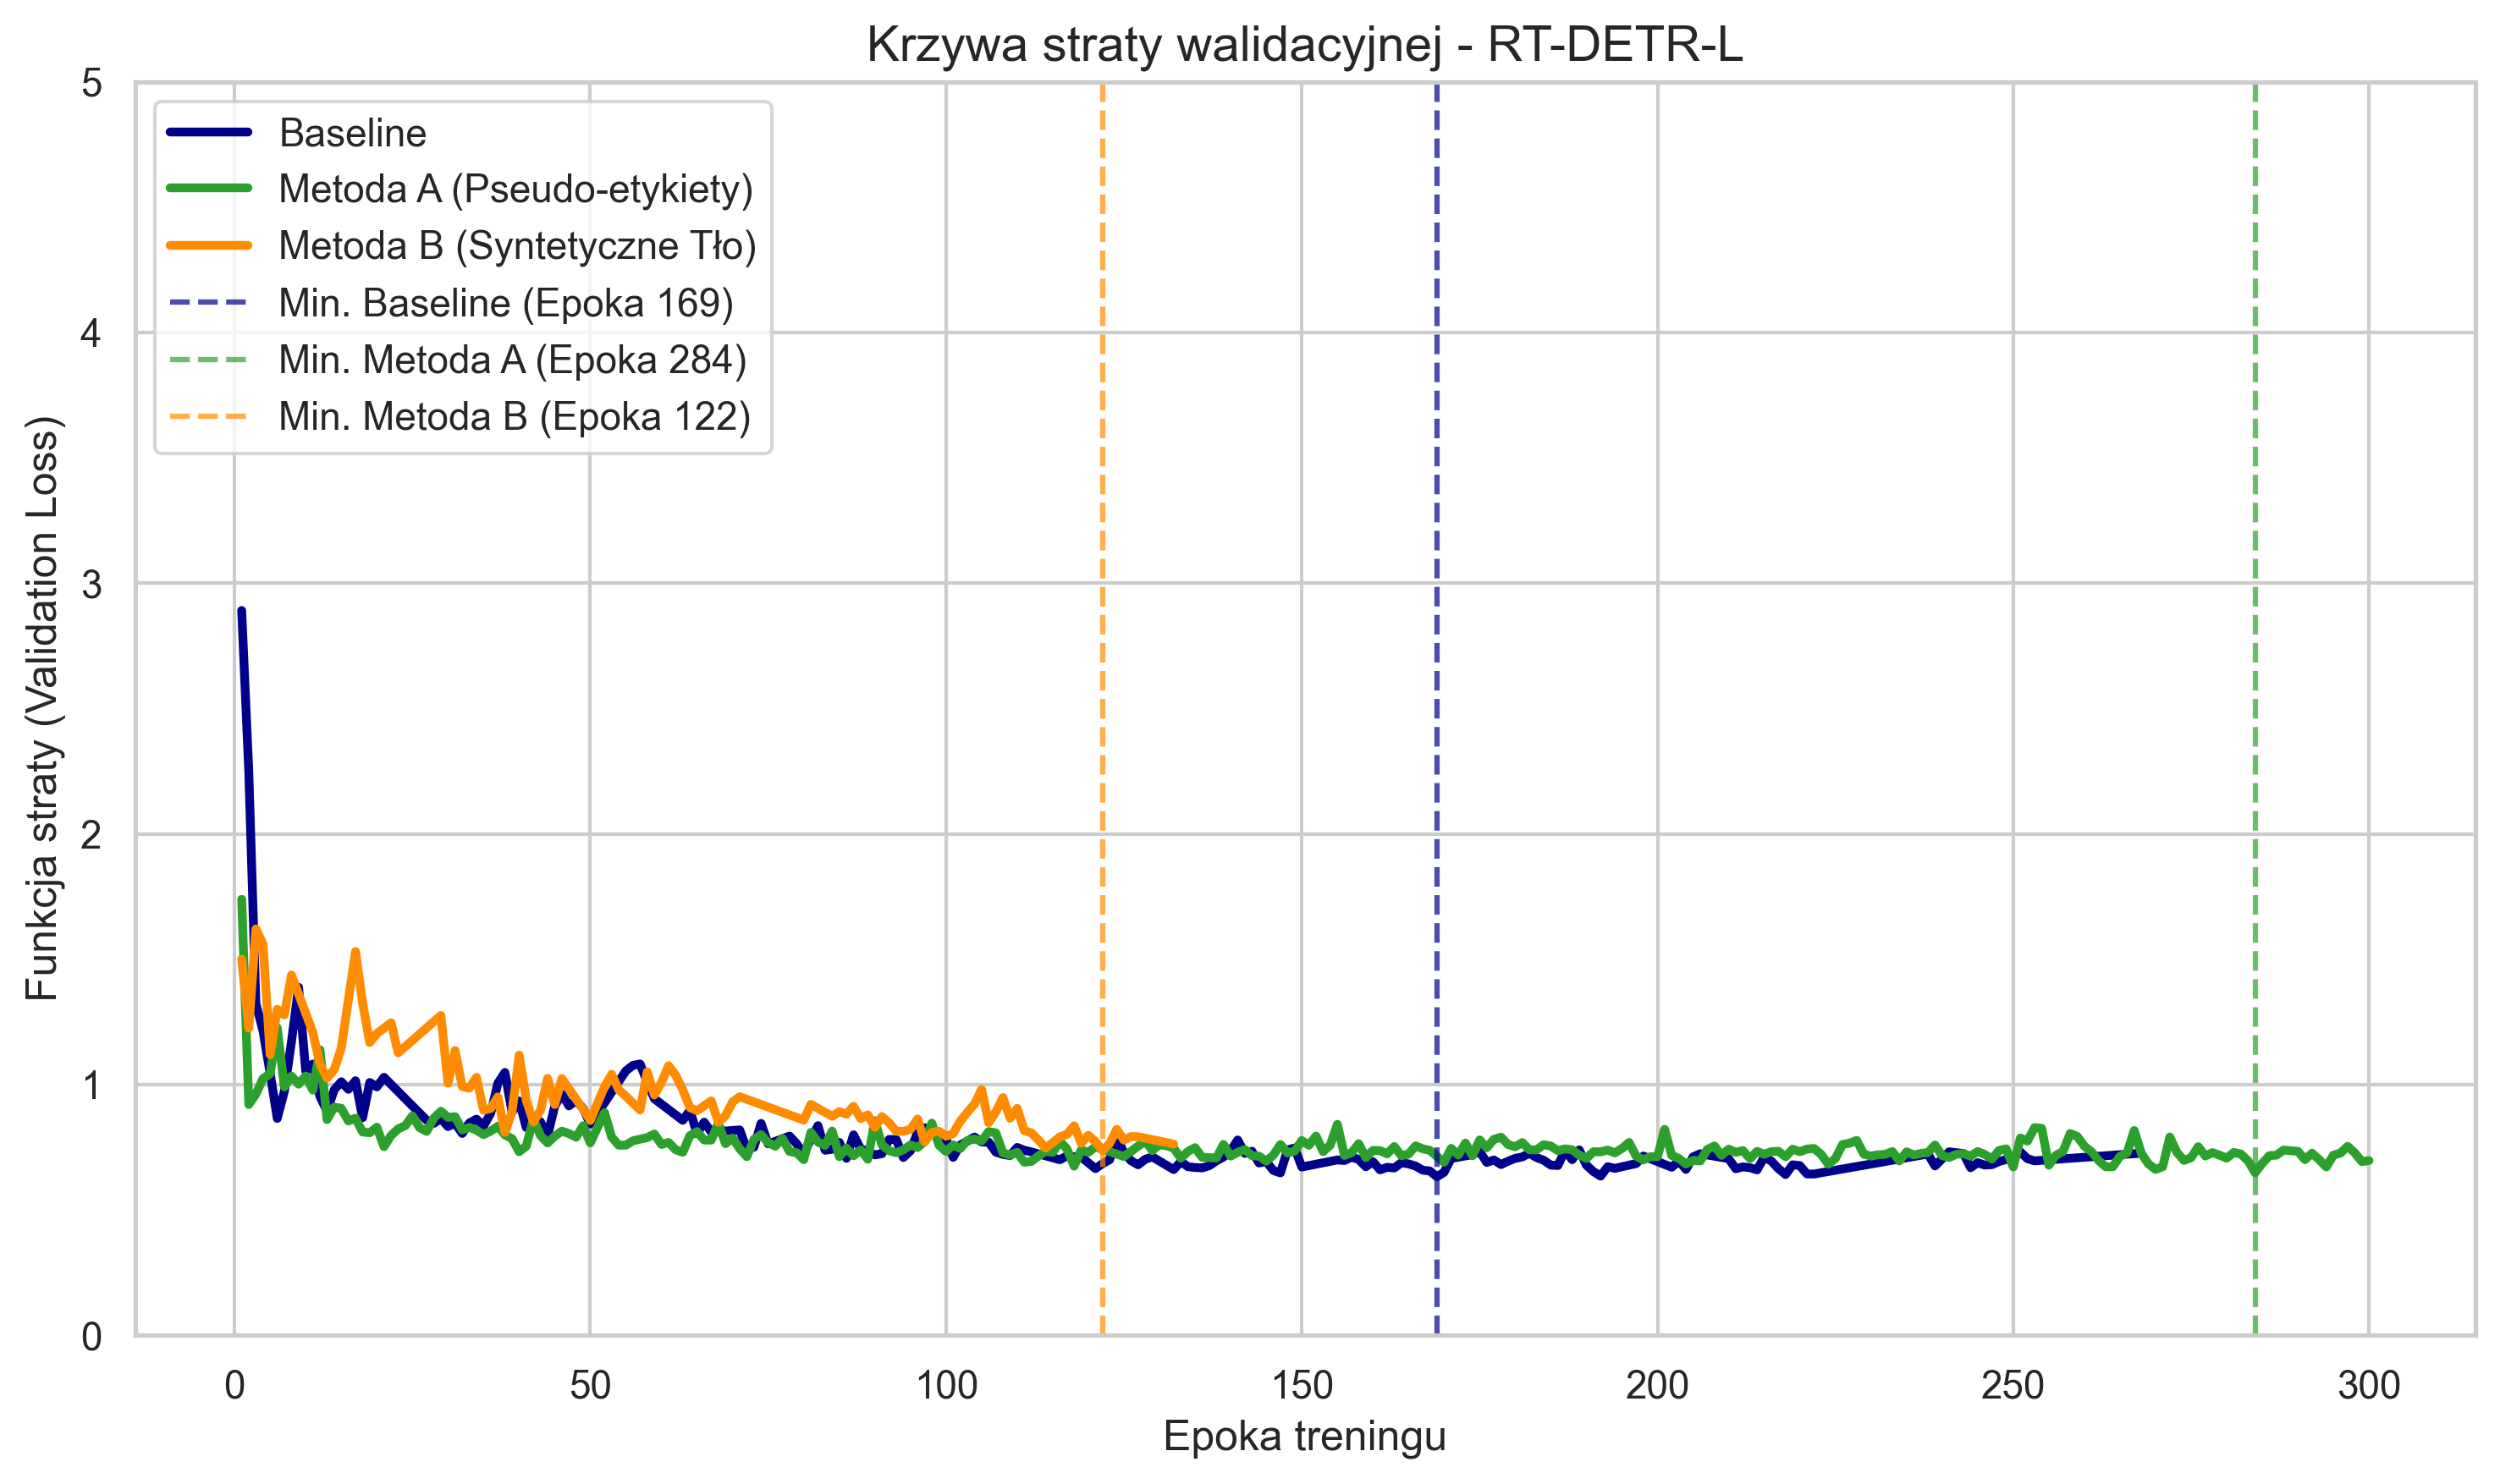
\includegraphics[width=1\linewidth]{Pics/Charts/wykres_2_loss_RT-DETR-L.png}
\caption{Krzywa straty dla danych ze zbioru walidacyjnego -- RT-DETR-L.}
\label{fig:loss_rtdetr}
\end{figure}

\section{Eksperyment A: Uczenie półnadzorowane (SSL Pseudo)}

W~odpowiedzi na ograniczenia zidentyfikowane w~modelach odniesienia zastosowano iteracyjne uczenie półnadzorowane. W~Metodzie A~(oznaczonej jako SSL Pseudo) wykorzystano surowe dane nieoznakowane, które przechodziły przez cykl generowania pseudoetykiet w~architekturze Nauczyciel--Uczeń.

\subsection{Wyniki dla architektury YOLOv8n i~YOLOv26n}

Proces iteracyjnego uczenia z~pseudoetykietami przyniósł odmienne rezultaty dla obu wariantów YOLO. Jak wskazuje wykres podatności architektur (Rysunek \ref{fig:susceptibility}), wdrożenie tej metody spowodowało spadek parametru mAP@0.5 dla modelu YOLOv8n o~2.3 p.p. względem modelu odniesienia. O~ile czułość modelu wzrosła do 0.811, to precyzja spadła do 0.812. Można to interpretować jako skutek błędu potwierdzenia (\emph{confirmation bias}) -- niedoskonałe pseudoetykiety wygenerowane w~pierwszych iteracjach potoku SSL wprowadziły szum, który zwiększył liczbę mniej precyzyjnych wskazań. Minimum funkcji straty walidacyjnej przesunęło się z~256. do 275. epoki (Rysunek \ref{fig:loss_yolo8}).

Inaczej zareagował model YOLOv26n. Zastosowanie metody SSL Pseudo pozwoliło mu poprawić mAP@0.5 o~3.4 p.p. (wzrost do 0.857). Zarówno precyzja, jak i~czułość uległy poprawie. Przetworzenie dodatkowych, nieoznakowanych danych w~pętli Nauczyciel--Uczeń zadziałało w~tym przypadku jak mechanizm regularyzacji. Dodanie tych danych przesunęło minimum funkcji straty z~233. na 283. epokę (Rysunek \ref{fig:loss_yolo26}).

% MIEJSCE NA KRZYWE UCZENIA mAP (YOLO)
\begin{figure}[htbp]
\centering
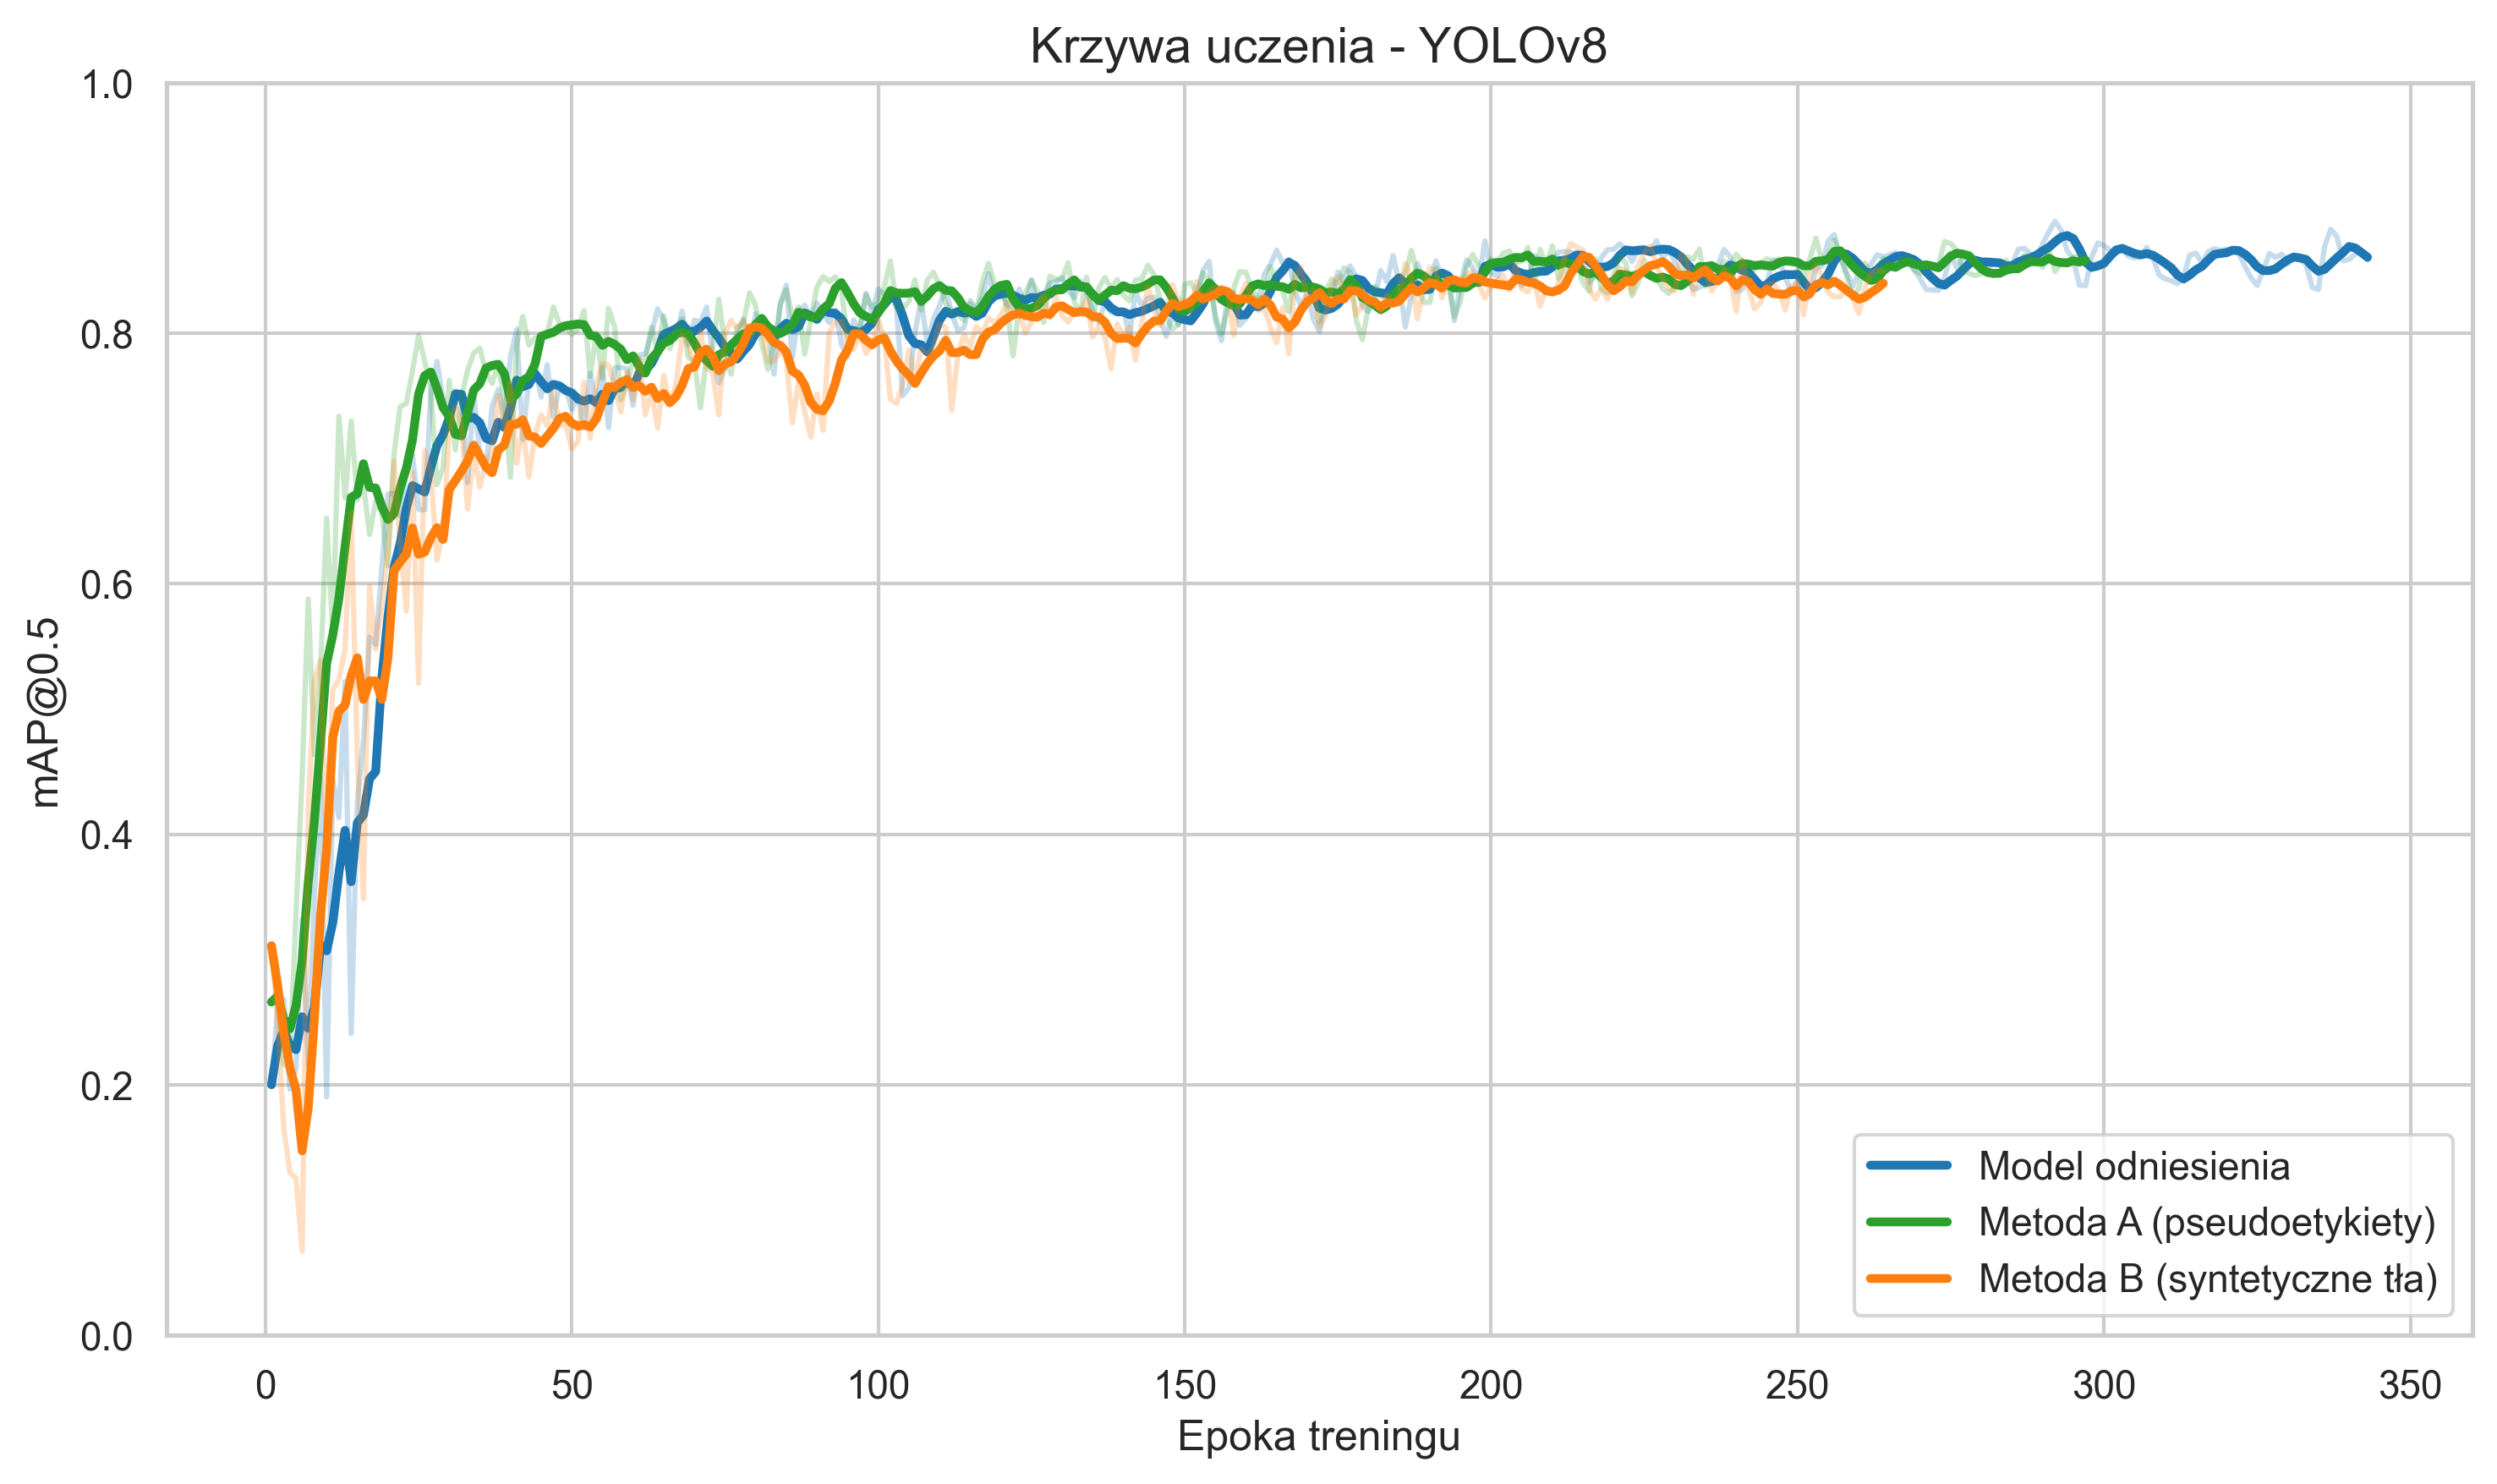
\includegraphics[width=1\linewidth]{Pics/Charts/wykres_4_konwergencja_YOLOv8.png}
\caption{Krzywa uczenia metryki mAP@0.5 dla modelu YOLOv8n na zbiorze walidacyjnym.}
\label{fig:map_yolo8}
\end{figure}

\begin{figure}[htbp]
\centering
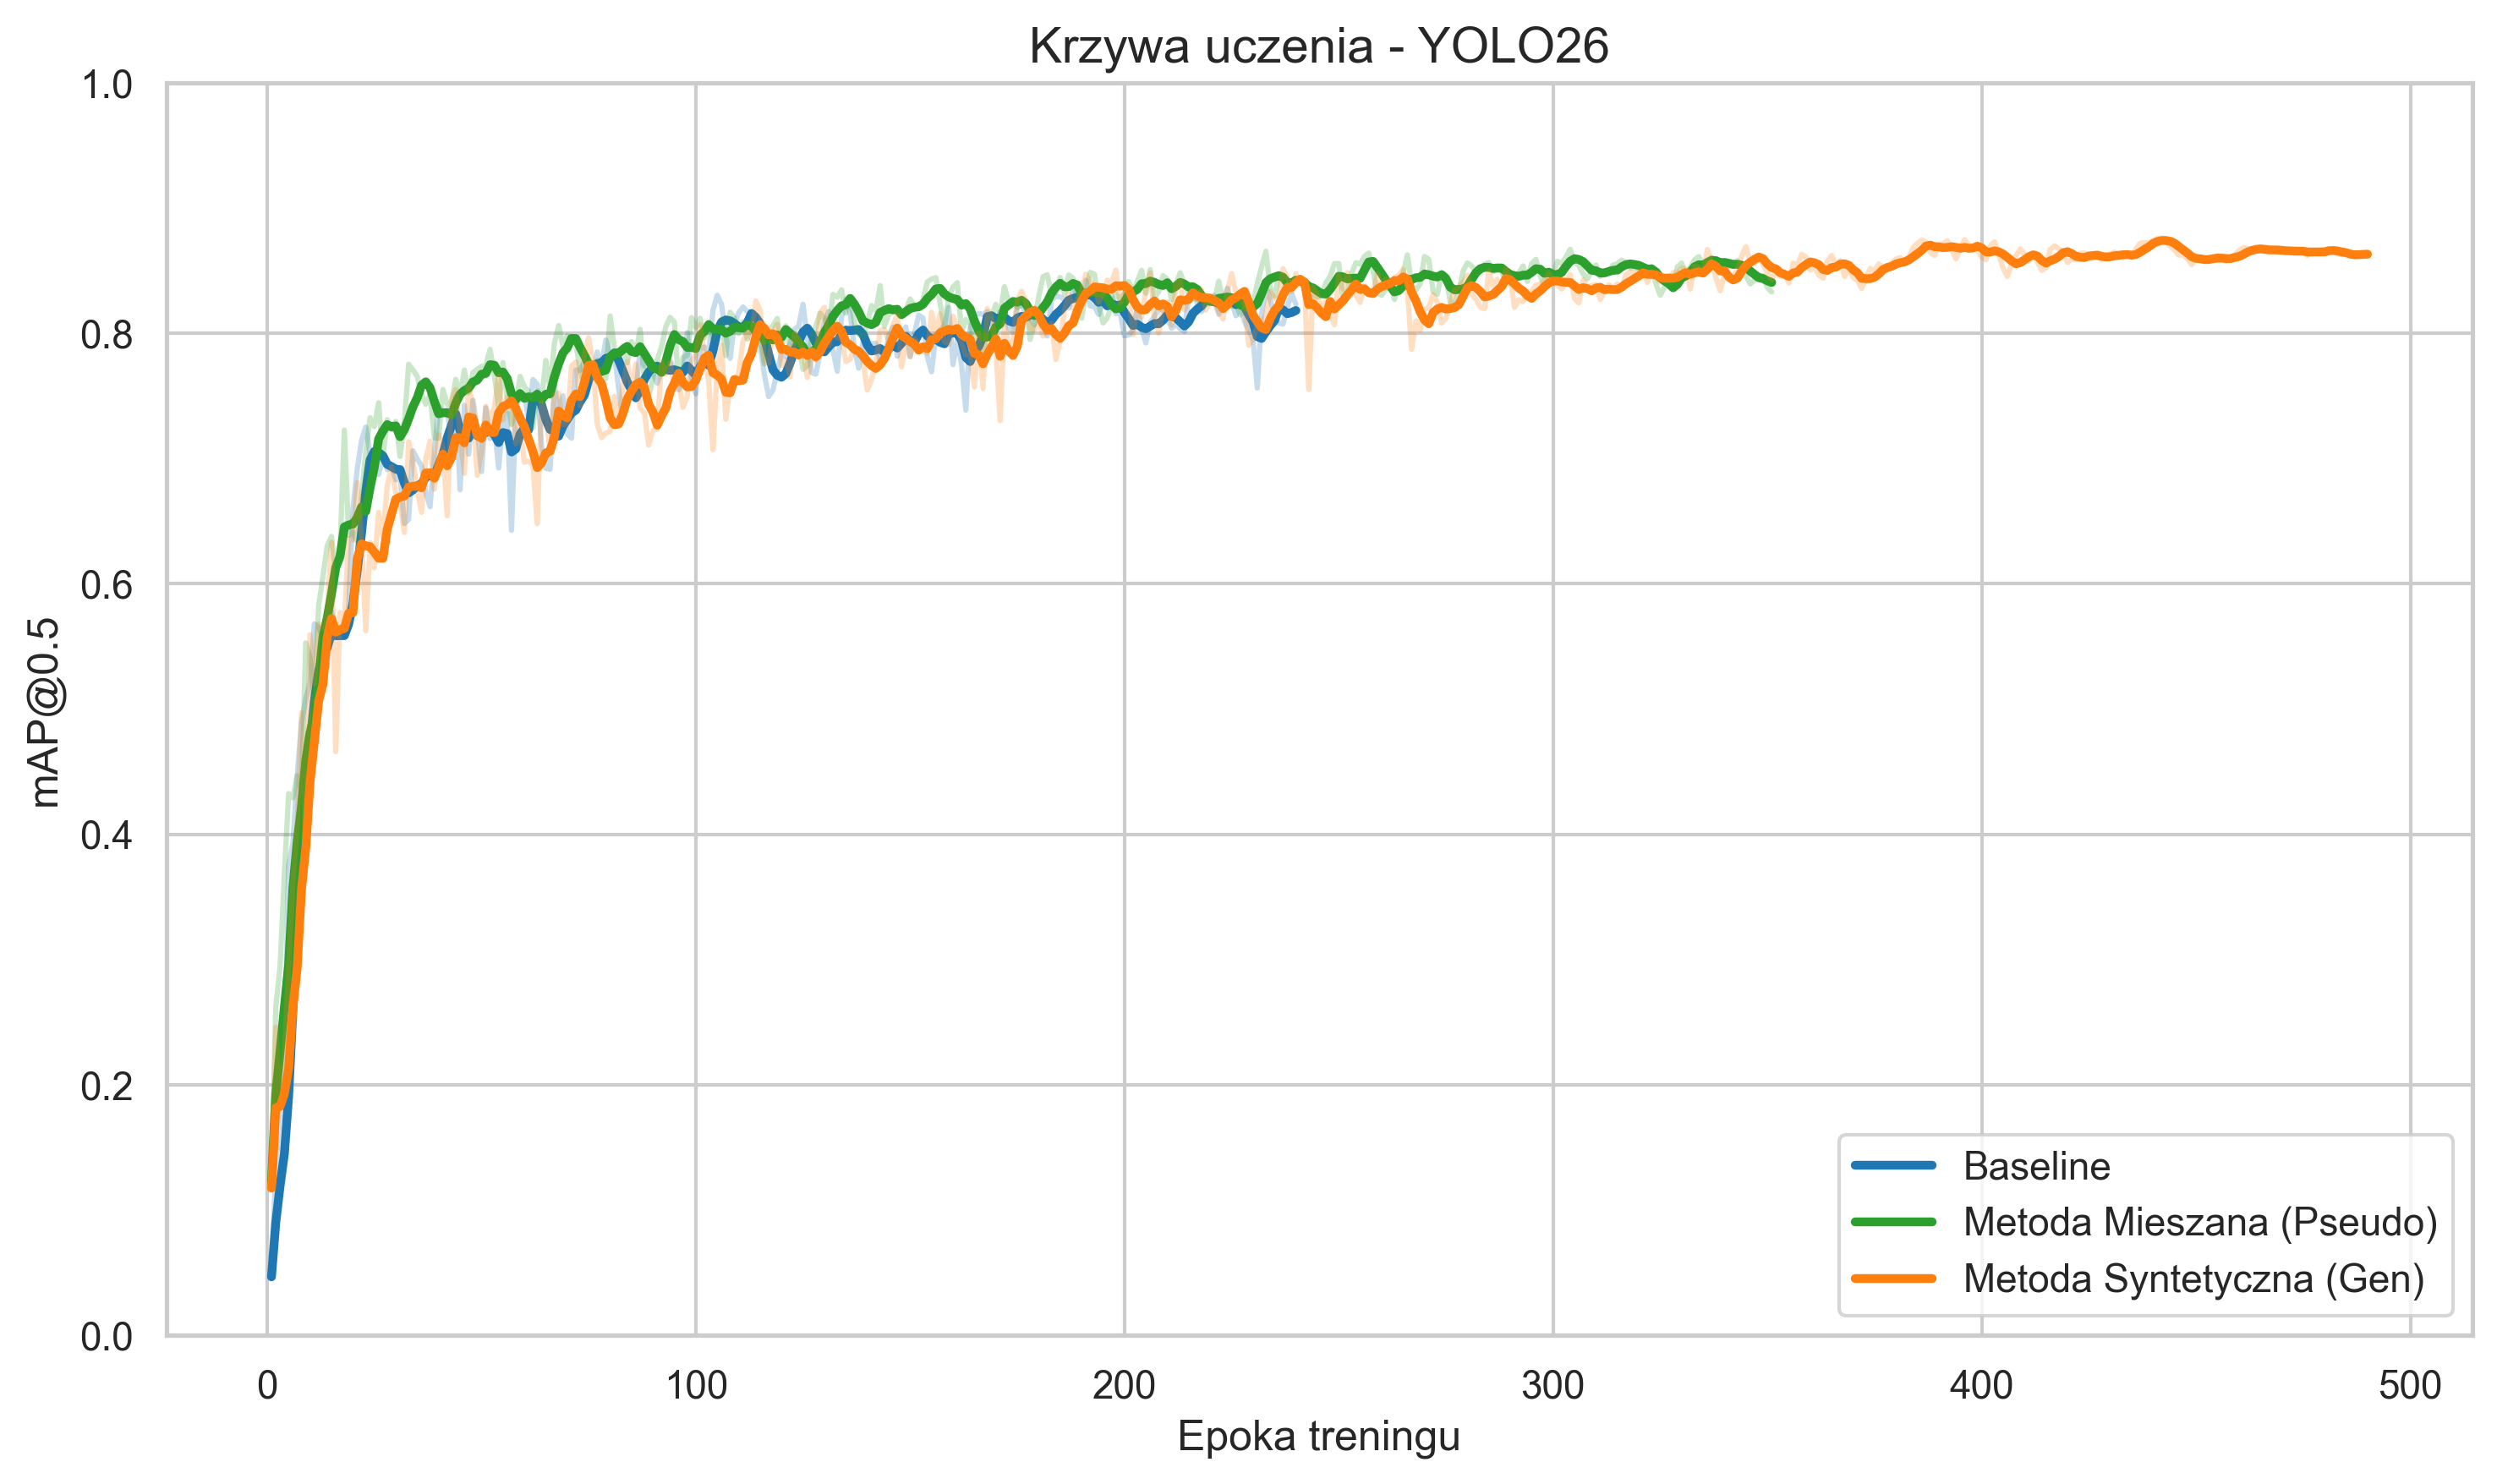
\includegraphics[width=1\linewidth]{Pics/Charts/wykres_4_konwergencja_YOLO26.png}
\caption{Krzywa uczenia metryki mAP@0.5 dla modelu YOLOv26n na zbiorze walidacyjnym.}
\label{fig:map_yolo26}
\end{figure}

\subsection{Wyniki dla architektury RT-DETR-L}

Dla detektora RT-DETR-L wdrożenie Metody A~przyniosło niewielki wzrost globalnej metryki mAP@0.5 (+0.3 p.p., do poziomu 0.880), jednak istotna była również zmiana relacji między precyzją i~czułością. Obie metryki wzrosły względem modelu odniesienia, co przełożyło się na najwyższy wynik F1 dla tej architektury.

Z~analizy krzywej uczenia (mAP na przestrzeni epok, Rysunek \ref{fig:map_rtdetr}) dla RT-DETR-L wynika, że zastosowanie SSL Pseudo pozwoliło utrzymać wysoką jakość detekcji przy niewielkiej poprawie metryk końcowych. Jednocześnie minimum straty walidacyjnej wystąpiło wcześniej niż dla modelu odniesienia (126. epoka wobec 230. epoki), co wskazuje, że dodatkowe dane nie przełożyły się w~tym przypadku na późniejsze minimum funkcji straty, mimo poprawy F1-score.

% MIEJSCE NA KRZYWĄ UCZENIA mAP (RT-DETR)
\begin{figure}[htbp]
\centering
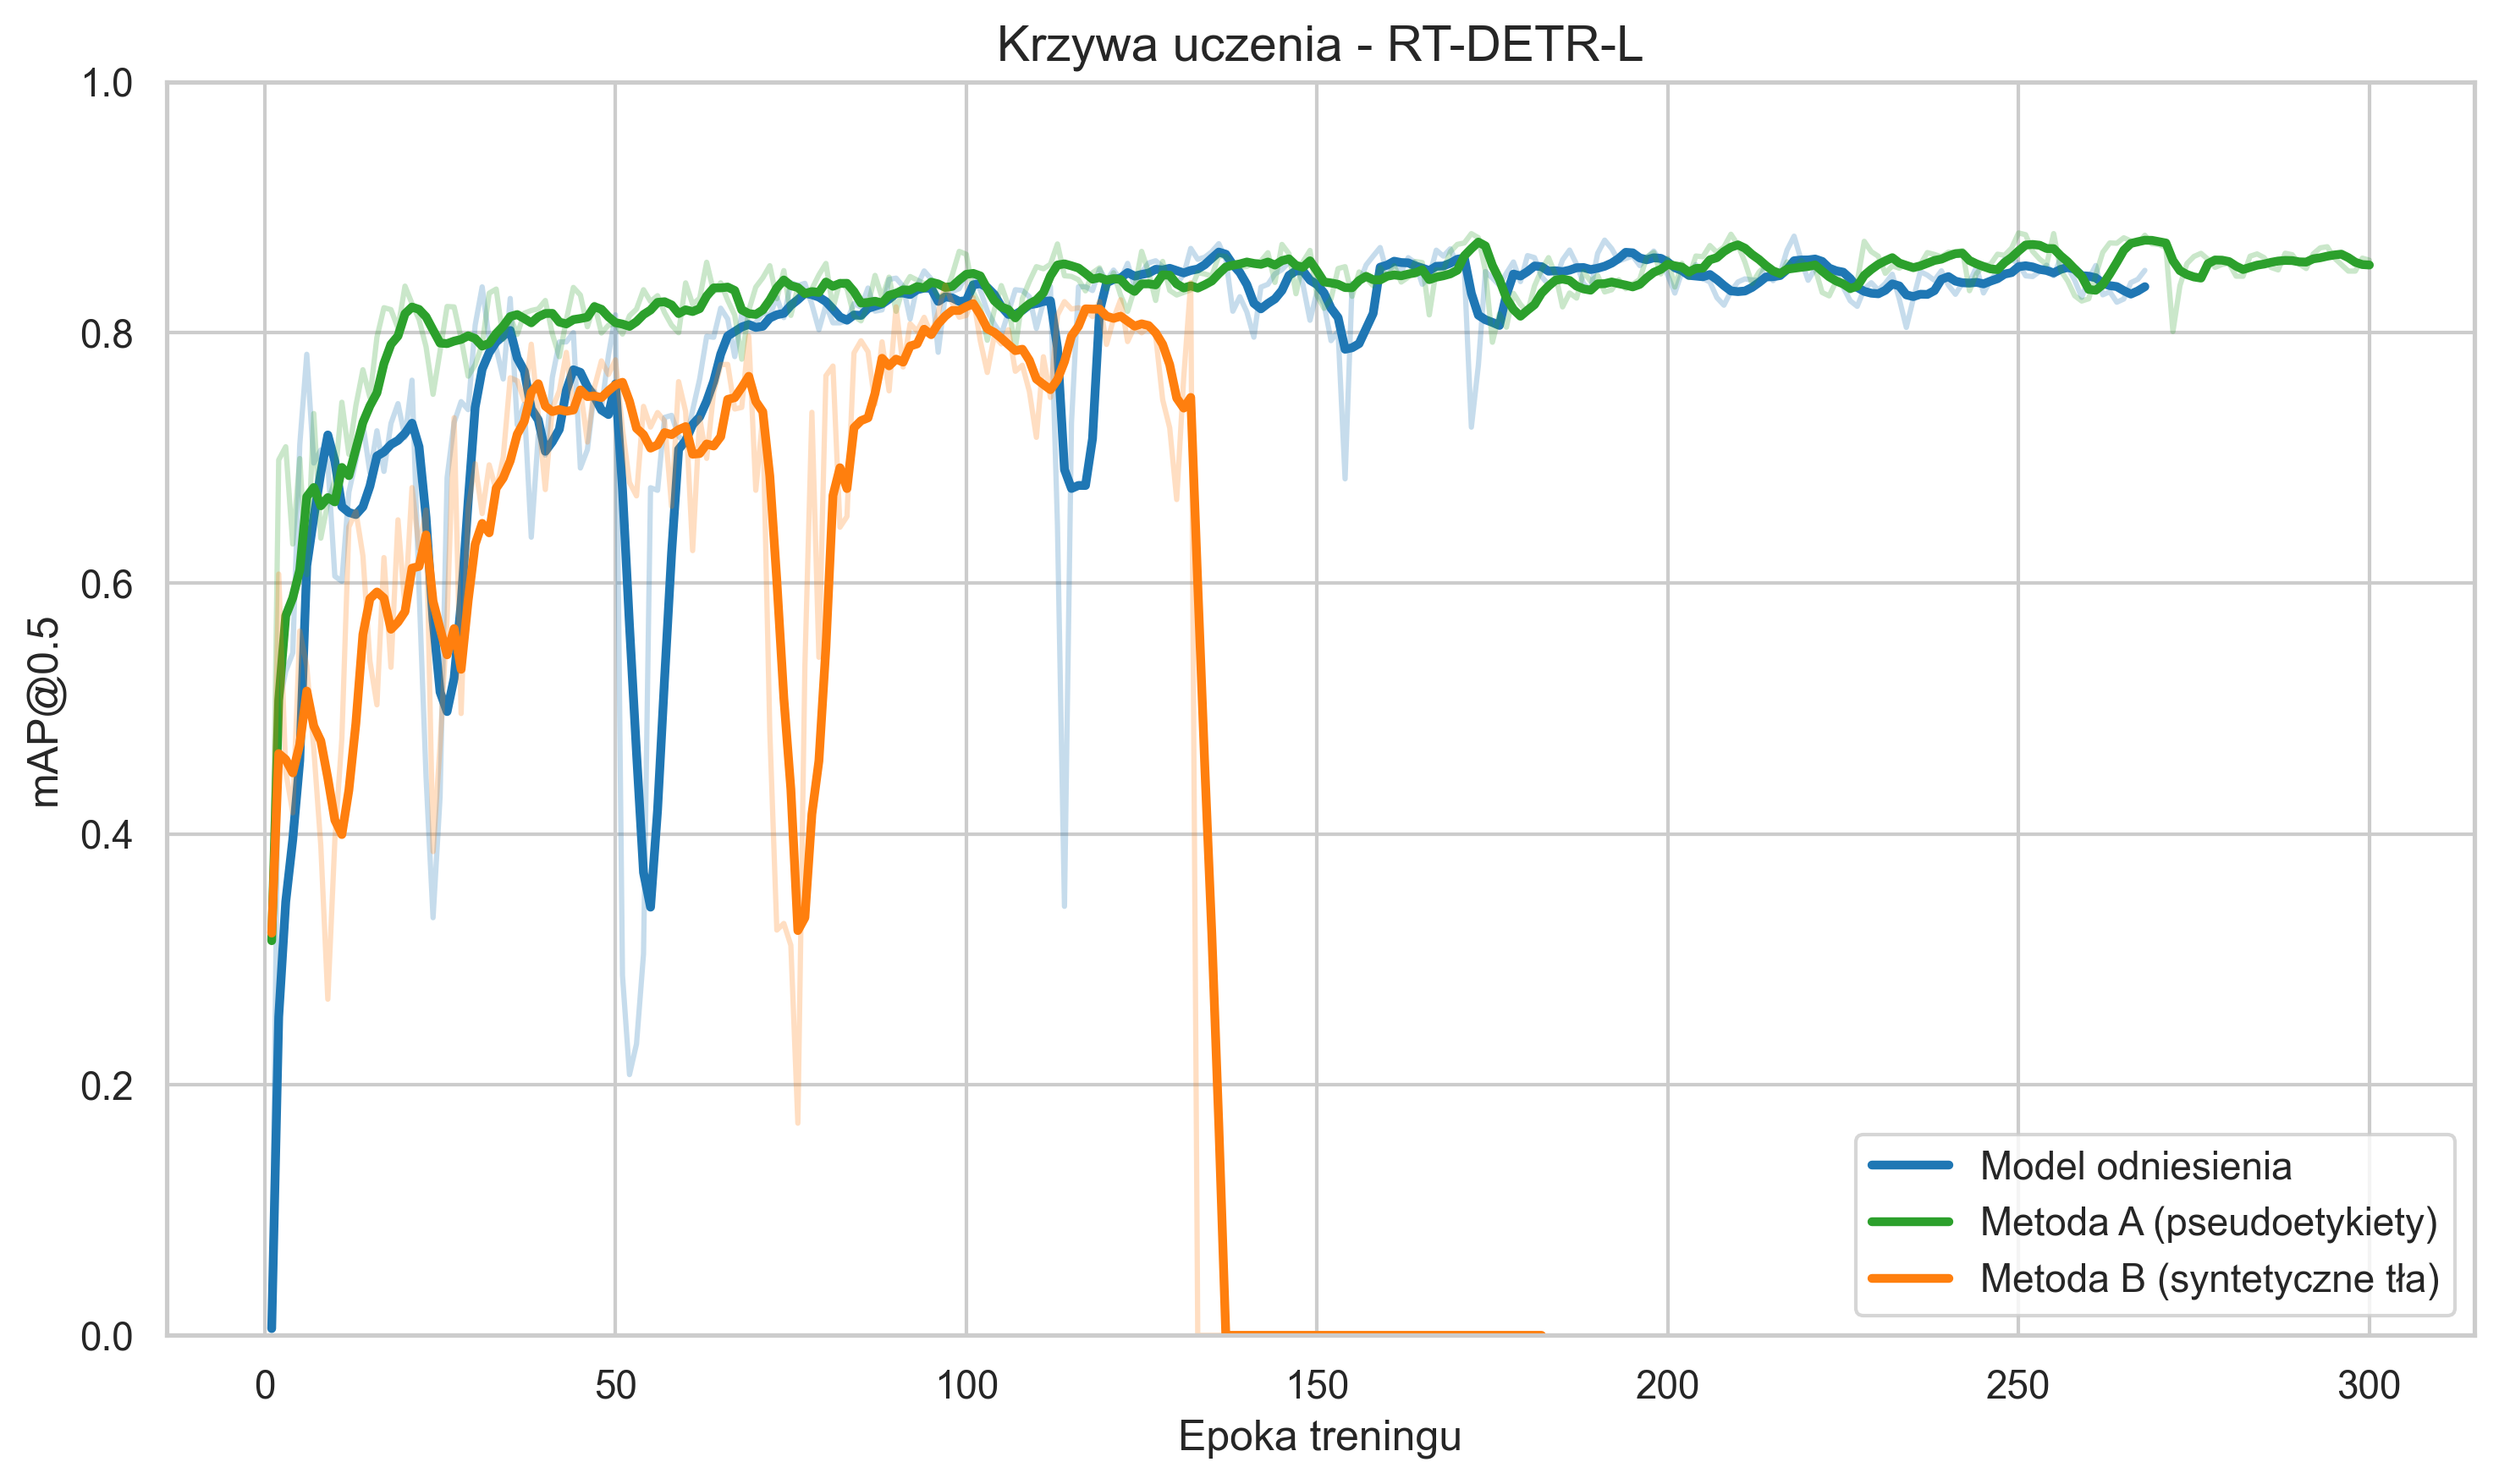
\includegraphics[width=1\linewidth]{Pics/Charts/wykres_4_konwergencja_RT-DETR-L.png}
\caption{Krzywa uczenia metryki mAP@0.5 dla modelu RT-DETR-L na zbiorze walidacyjnym.}
\label{fig:map_rtdetr}
\end{figure}

\section{Eksperyment B: Uczenie półnadzorowane z~syntetycznym tłem (SSL Generative)}

W~drugim eksperymencie proces SSL rozszerzono o~syntetycznie wygenerowane próbki negatywne (Metoda B). Do zbioru dodano obrazy przedstawiające różne typy tła bez obiektów docelowych. Rozwiązanie to miało zwiększyć różnorodność danych treningowych i~ograniczyć liczbę fałszywych detekcji związanych z~przeuczeniem modelu na konkretnych fragmentach tła.

\subsection{Analiza wyników dla modeli YOLO}

Dodanie syntetycznie wygenerowanych próbek negatywnych do procesu SSL nie poprawiło skuteczności modelu YOLOv8n względem modelu odniesienia (spadek mAP@0.5 o~1.4 p.p.). Precyzja wzrosła do 0.867, ale czułość obniżyła się do 0.724. Wyniki sugerują, że model stał się bardziej konserwatywny w~generowaniu detekcji, co ograniczyło część fałszywych wskazań, ale jednocześnie zwiększyło liczbę pominiętych obiektów.

Odmiennie zachował się model YOLOv26n, który w~tym eksperymencie osiągnął najlepsze wyniki spośród wszystkich wariantów tej architektury. Zastosowanie metody SSL Generative zwiększyło wartość mAP@0.5 o~5.1 p.p., osiągając wynik 0.874. Poprawie uległy również precyzja i~F1-score. Dodatkowe próbki negatywne mogły przyczynić się do lepszego rozróżniania obiektów docelowych od tła. Na ograniczenie przeuczenia może wskazywać przesunięcie minimum straty walidacyjnej z~233. na 445. epokę treningu (Rysunek \ref{fig:loss_yolo26}).

\subsection{Analiza wyników dla RT-DETR-L}

Dla architektury RT-DETR-L wykorzystanie potoku SSL rozszerzonego o~dane syntetyczne nie przyniosło poprawy wyników i~spowodowało spadek skuteczności detekcji. Model odnotował największy spadek mAP@0.5 w~całym zestawieniu (-3.7 p.p. względem modelu odniesienia, osiągając 0.840). 

Dodatkowo analiza krzywej uczenia modelu RT-DETR-L (Rysunek \ref{fig:map_rtdetr}) wskazuje, że w~przypadku Metody B proces treningu był mniej stabilny niż w~pozostałych wariantach. W~okolicach 135. epoki metryka mAP dla tego wariantu wyraźnie spadła, co pokrywa się z~pogorszeniem jakości końcowej. Wyniki te sugerują, że syntetyczne tła wprowadziły przesunięcie domenowe, na które architektura transformerowa okazała się bardziej wrażliwa niż modele YOLO.

\section{Wybrane przykłady predykcji}

Poniżej przedstawiono przykładowe predykcje modeli dla obrazów z~wyizolowanego zbioru \emph{Test-Sacred}, które nie były wykorzystywane na żadnym etapie treningu ani walidacji. Przykłady te służą wizualnej weryfikacji zdolności modeli do generalizacji poza zbiorem walidacyjnym. Dodatkowe przykłady zamieszczono w~Dodatku A. W~tabelach przedstawiono liczbę wszystkich detekcji, detekcji poprawnych (TP), fałszywie pozytywnych (FP) oraz fałszywie negatywnych (FN) dla pokazanego kafelka, przy progu IoU równym $0.5$.

\subsection{Predykcje modeli odniesienia}
\begin{figure}[htbp]
    \centering
    \subfloat[][YOLOv8n]{
    
\includegraphics[width = 0.3\textwidth]{Pics/Predictions/Sacred/YOLO8/Baseline/sacred_1_R001_C003.jpg}
    \label{fig:baseline_yolov8n}}
    \quad
    \subfloat[][YOLOv26n]{
    
\includegraphics[width = 0.3\textwidth]{Pics/Predictions/Sacred/YOLO26/Baseline/sacred_1_R001_C003.jpg}
    \label{fig:baseline_yolov26n}}
    \quad
    \subfloat[][RT-DETR-L]{
    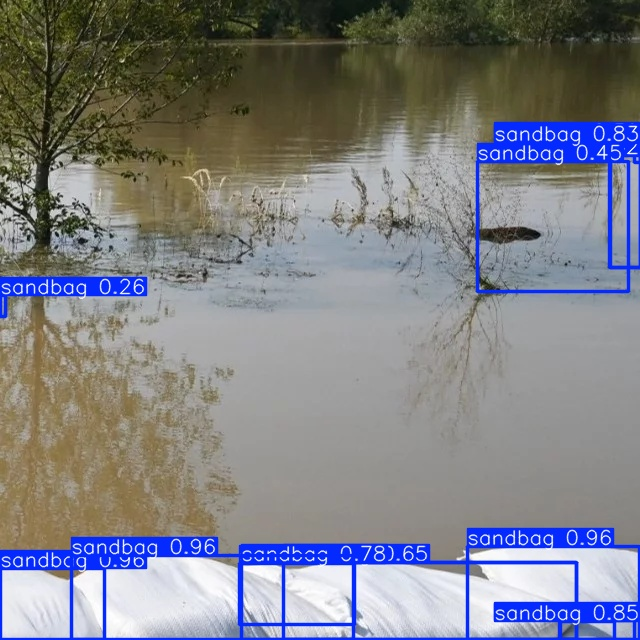
\includegraphics[width = 0.3\textwidth]{Pics/Predictions/Sacred/RT-DETR-L/Baseline/sacred_1_R001_C003.jpg}
    \label{fig:baseline_rtdetr}}
\caption{Porównanie predykcji modeli odniesienia dla obrazu ze zbioru \emph{Test-Sacred}.}
    \label{fig:baseline_comparison}
\end{figure}

\begin{table}[htbp]
\centering
\caption{Liczba detekcji, TP, FP i~FN dla modeli odniesienia na obrazie z~rysunku \ref{fig:baseline_comparison}.}
\label{tab:baseline_stats}
\begin{tabular}{|c|c|c|c|}
\hline
\textbf{Metryka} & \textbf{YOLOv8n} & \textbf{YOLOv26n} & \textbf{RT-DETR-L} \\ \hline
Liczba detekcji   & 14               & 6                 & 13                 \\ \hline
TP                & 0                & 0                 & 0                  \\ \hline
FP                & 14               & 6                 & 13                 \\ \hline
FN                & 4                & 4                 & 4                  \\ \hline
Precyzja          & 0.00             & 0.00              & 0.00               \\ \hline
Czułość           & 0.00             & 0.00              & 0.00               \\ \hline
\end{tabular}
\end{table}

Analiza rysunku \ref{fig:baseline_comparison} oraz danych ilościowych z~tabeli \ref{tab:baseline_stats} pokazuje, że wybrany kafelek jest trudnym przypadkiem dla modeli odniesienia. Modele generują wiele wskazań, ale nie pokrywają one poprawnie czterech obiektów referencyjnych przy progu IoU równym $0.5$. Szczególnie widoczne jest to dla YOLOv8n oraz RT-DETR-L, które wskazały odpowiednio 14 i~13 fałszywie pozytywnych detekcji.

\subsection{Predykcje modeli z~Metody A~(SSL Pseudo)}
\begin{figure}[htbp]
    \centering
    \subfloat[][YOLOv8n]{
    
\includegraphics[width = 0.3\textwidth]{Pics/Predictions/Sacred/YOLO8/Pseudo/sacred_1_R001_C003.jpg}
    \label{fig:pseudo_yolov8n}}
    \quad
    \subfloat[][YOLOv26n]{
    
\includegraphics[width = 0.3\textwidth]{Pics/Predictions/Sacred/YOLO26/Pseudo/sacred_1_R001_C003.jpg}
    \label{fig:pseudo_yolov26n}}
    \quad
    \subfloat[][RT-DETR-L]{
    
\includegraphics[width = 0.3\textwidth]{Pics/Predictions/Sacred/RT-DETR-L/Pseudo/sacred_1_R001_C003.jpg}
    \label{fig:pseudo_rtdetr}}
\caption{Porównanie predykcji modeli po zastosowaniu pseudoetykietowania dla obrazu ze zbioru \emph{Test-Sacred}.}
    \label{fig:pseudo_comparison}
\end{figure}

\begin{table}[htbp]
\centering
\caption{Liczba detekcji, TP, FP i~FN dla metody SSL Pseudo na obrazie z~rysunku \ref{fig:pseudo_comparison}.}
\label{tab:pseudo_stats}
\begin{tabular}{|c|c|c|c|}
\hline
\textbf{Metryka} & \textbf{YOLOv8n} & \textbf{YOLOv26n} & \textbf{RT-DETR-L} \\ \hline
Liczba detekcji     & 7                & 6                 & 7                  \\ \hline
TP                  & 0                & 0                 & 0                  \\ \hline
FP                  & 7                & 6                 & 7                  \\ \hline
FN                  & 4                & 4                 & 4                  \\ \hline
Precyzja            & 0.00             & 0.00              & 0.00               \\ \hline
Czułość             & 0.00             & 0.00              & 0.00               \\ \hline
\end{tabular}
\end{table}


Zastosowanie iteracyjnego pseudoetykietowania zmniejszyło liczbę wskazań dla modeli YOLOv8n i~RT-DETR-L, co ograniczyło liczbę fałszywie pozytywnych detekcji na analizowanym kafelku. Jednocześnie żaden z~modeli nie uzyskał poprawnego dopasowania do ramek referencyjnych przy progu IoU $0.5$, dlatego przykład ten należy interpretować jako ilustrację redukcji nadmiarowych wskazań, a~nie pełnej poprawy lokalizacji obiektów.

\subsection{Predykcje modeli z~Metody B (SSL Generative)}
\begin{figure}[htbp]
    \centering
    \subfloat[][YOLOv8n]{
    
\includegraphics[width = 0.3\textwidth]{Pics/Predictions/Sacred/YOLO8/Generative/sacred_1_R001_C003.jpg}
    \label{fig:generative_yolov8n}}
    \quad
    \subfloat[][YOLOv26n]{
    
\includegraphics[width = 0.3\textwidth]{Pics/Predictions/Sacred/YOLO26/Generative/sacred_1_R001_C003.jpg}
    \label{fig:generative_yolov26n}}
    \quad
    \subfloat[][RT-DETR-L]{
    
\includegraphics[width = 0.3\textwidth]{Pics/Predictions/Sacred/RT-DETR-L/Generative/sacred_1_R001_C003.jpg}
    \label{fig:generative_rtdetr}}
\caption{Porównanie predykcji modeli po włączeniu syntetycznych próbek tła dla obrazu ze zbioru \emph{Test-Sacred}.}
    \label{fig:generative_comparison}
\end{figure}

\begin{table}[htbp]
\centering
\caption{Liczba detekcji, TP, FP i~FN dla metody SSL Generative na obrazie z~rysunku \ref{fig:generative_comparison}.}
\label{tab:generative_stats}
\begin{tabular}{|c|c|c|c|}
\hline
\textbf{Metryka} & \textbf{YOLOv8n} & \textbf{YOLOv26n} & \textbf{RT-DETR-L} \\ \hline
Liczba detekcji         & 7                & 5                 & 17                 \\ \hline
TP                      & 0                & 0                 & 0                  \\ \hline
FP                      & 7                & 5                 & 17                 \\ \hline
FN                      & 4                & 4                 & 4                  \\ \hline
Precyzja                & 0.00             & 0.00              & 0.00               \\ \hline
Czułość                 & 0.00             & 0.00              & 0.00               \\ \hline
\end{tabular}
\end{table}

Dodanie syntetycznych obrazów tła (Metoda B) uwidoczniło różnice w~zachowaniu poszczególnych architektur. Dla modeli YOLO liczba wskazań pozostała niższa niż w~modelach odniesienia, co sugeruje działanie próbek negatywnych jako dodatkowego mechanizmu ograniczającego nadmiarowe detekcje.

Odmienne zachowanie zaobserwowano dla modelu RT-DETR-L. Wprowadzenie syntetycznych danych zwiększyło liczbę fałszywie pozytywnych wskazań do 17, co jest spójne z~wynikami ilościowymi pokazującymi pogorszenie metryk tej architektury po zastosowaniu Metody B. Jedną z~możliwych przyczyn jest uczenie się zależności obecnych w~danych syntetycznych, które nie występowały w~danych rzeczywistych.

\section{Analiza statystyczna fałszywych detekcji}

W~celu obiektywnej weryfikacji skuteczności zastosowanych technik SSL (pseudoetykietowanie oraz syntetyczne próbki tła), przeprowadzono analizę statystyczną różnic w~liczbie fałszywych detekcji. Głównym celem tej analizy było sprawdzenie, czy proponowane metody redukują liczbę fałszywie pozytywnych wskazań modelu, co stanowi jeden z~kluczowych problemów w~reżimie małego zbioru danych.
\subsection{Metodyka testów}
Podstawowym wyzwaniem w~standardowej analizie agregowanej (np. globalnym mAP) jest fakt, że eksperymenty typu \textit{single-seed} dostarczają tylko jednego wyniku zbiorczego, co ogranicza moc statystyczną oceny. W~niniejszej pracy wyliczono liczbę fałszywych detekcji (FP) osobno dla każdego z~43 kadrów walidacyjnych. Dzięki takiemu podejściu uzyskano dla każdego modelu wektor obserwacji, co umożliwiło przeprowadzenie testów nieparametrycznych.
Ze względu na niespełnienie założeń o~rozkładzie normalnym wyników oraz charakter prób powiązanych (ten sam zbiór walidacyjny dla modeli odniesienia i~wariantów SSL), zastosowano jednostronny test znakowanych rang Wilcoxona. Test wykonano w~bibliotece \texttt{scipy.stats}, sprawdzając, czy zastosowana metoda redukuje liczbę fałszywych detekcji względem modelu odniesienia. Za próg istotności statystycznej przyjęto wartość $p < 0.05$.

\subsection{Wyniki analizy}
Zestawienie wyników testu statystycznego przedstawiono w~Tabeli \ref{tab:stat_analysis}.

\begin{table}[htbp]
\centering
\caption{Analiza statystyczna redukcji liczby fałszywych detekcji (FP) na zbiorze walidacyjnym przy użyciu testu Wilcoxona.}
\label{tab:stat_analysis}
\resizebox{\textwidth}{!}{%
\begin{tabular}{|l|l|c|c|c|c|}
\hline
\textbf{Architektura} & \textbf{Porównanie} & \textbf{Śr. FP (odnies.)} & \textbf{Śr. FP (metoda)} & \textbf{Wartość $p$} & \textbf{Istotność ($p<0.05$)} \\ \hline
\multirow{2}{*}{\textbf{YOLOv8}}
 & Odniesienie vs SSL Pseudo & 13.37 & 11.88 & 0.0030 & TAK \\ \cline{2-6} 
 & Odniesienie vs SSL Generative & 13.37 & 11.93 & 0.0012 & TAK \\ \hline
\multirow{2}{*}{\textbf{YOLOv26}}
 & Odniesienie vs SSL Pseudo & 10.00 & 10.88 & 0.9652 & NIE \\ \cline{2-6} 
 & Odniesienie vs SSL Generative & 10.00 & 10.91 & 0.9626 & NIE \\ \hline
\multirow{2}{*}{\textbf{RT-DETR-L}}
 & Odniesienie vs SSL Pseudo & 15.51 & 14.14 & 0.0103 & TAK \\ \cline{2-6} 
 & Odniesienie vs SSL Generative & 15.51 & 20.23 & 0.9997 & NIE \\ \hline
\end{tabular}%
}
\end{table}
Uzyskane wyniki wskazują na zróżnicowaną podatność architektur na zastosowane metody. W~przypadku modelu YOLOv8n obie metody SSL przyniosły statystycznie istotną redukcję fałszywych detekcji ($p < 0.05$), co wspiera interpretację, że dodatkowe dane pełniły funkcję regularyzacyjną. W~modelu RT-DETR-L istotną redukcję osiągnięto jedynie przy użyciu metody SSL Pseudo. Brak istotnej redukcji dla metody SSL Generative w~architekturze RT-DETR-L ($p=0.9997$) jest spójny z~wcześniejszą obserwacją wzrostu liczby fałszywych wskazań po wprowadzeniu danych syntetycznych.

\section{Podsumowanie i~ostateczna analiza porównawcza}

Szczegółowe zestawienie wszystkich monitorowanych metryk ewaluacyjnych (w~tym parametru F1-score) oraz punktów krytycznych treningu (epoka wystąpienia minimum straty walidacyjnej) dla każdego z~badanych wariantów zaprezentowano w~Tabeli \ref{tab:final_results}. 

\begin{table}[htbp]
\centering
\caption{Szczegółowe zestawienie metryk ewaluacyjnych oraz epoki wystąpienia minimum funkcji straty na zbiorze walidacyjnym.}
\label{tab:final_results}
\resizebox{\textwidth}{!}{% Zmniejsza tabelę, jeśli wychodzi poza marginesy
\begin{tabular}{|c|l|c|c|c|c|c|c|}
\hline
\textbf{Architektura} & \textbf{Metoda} & \textbf{mAP@0.5} & \textbf{mAP@0.5:0.95} & \textbf{Precyzja} & \textbf{Czułość} & \textbf{F1-score} & \textbf{Min. straty (epoka)} \\ \hline
\multirow{3}{*}{\textbf{YOLOv8}}
 & Model odniesienia & \textbf{0.882} & \textbf{0.650} & 0.845 & 0.777 & 0.809 & 256 \\ \cline{2-8} 
 & Metoda A (Pseudo) & 0.859 & 0.623 & 0.812 & \textbf{0.811} & \textbf{0.812} & \textbf{275} \\ \cline{2-8} 
 & Metoda B (Generative) & 0.869 & 0.623 & \textbf{0.867} & 0.724 & 0.789 & 246 \\ \hline
\multirow{3}{*}{\textbf{YOLOv26}}
 & Model odniesienia & 0.823 & 0.592 & 0.807 & 0.737 & 0.770 & 233 \\ \cline{2-8} 
 & Metoda A (Pseudo) & 0.857 & 0.621 & 0.819 & \textbf{0.782} & 0.800 & 283 \\ \cline{2-8} 
 & Metoda B (Generative) & \textbf{0.874} & \textbf{0.643} & \textbf{0.851} & 0.766 & \textbf{0.806} & \textbf{445} \\ \hline
\multirow{3}{*}{\textbf{RT-DETR-L}}
 & Model odniesienia & 0.877 & \textbf{0.677} & 0.829 & 0.817 & 0.823 & \textbf{230} \\ \cline{2-8} 
 & Metoda A (Pseudo) & \textbf{0.880} & 0.675 & \textbf{0.844} & \textbf{0.830} & \textbf{0.837} & 126 \\ \cline{2-8} 
 & Metoda B (Generative) & 0.840 & 0.612 & 0.785 & 0.792 & 0.789 & 66 \\ \hline
\end{tabular}%
}
\end{table}


Zestawienie wyników ilościowych z~przykładami predykcji ze zbioru \emph{Test-Sacred} pozwala na sformułowanie wniosków dotyczących podatności badanych architektur na analizowane techniki. Na wykresie podatności można wyróżnić trzy różne profile zachowań sieci:

% MIEJSCE NA WYKRES PODATNOŚCI
\begin{figure}[htbp]
\centering
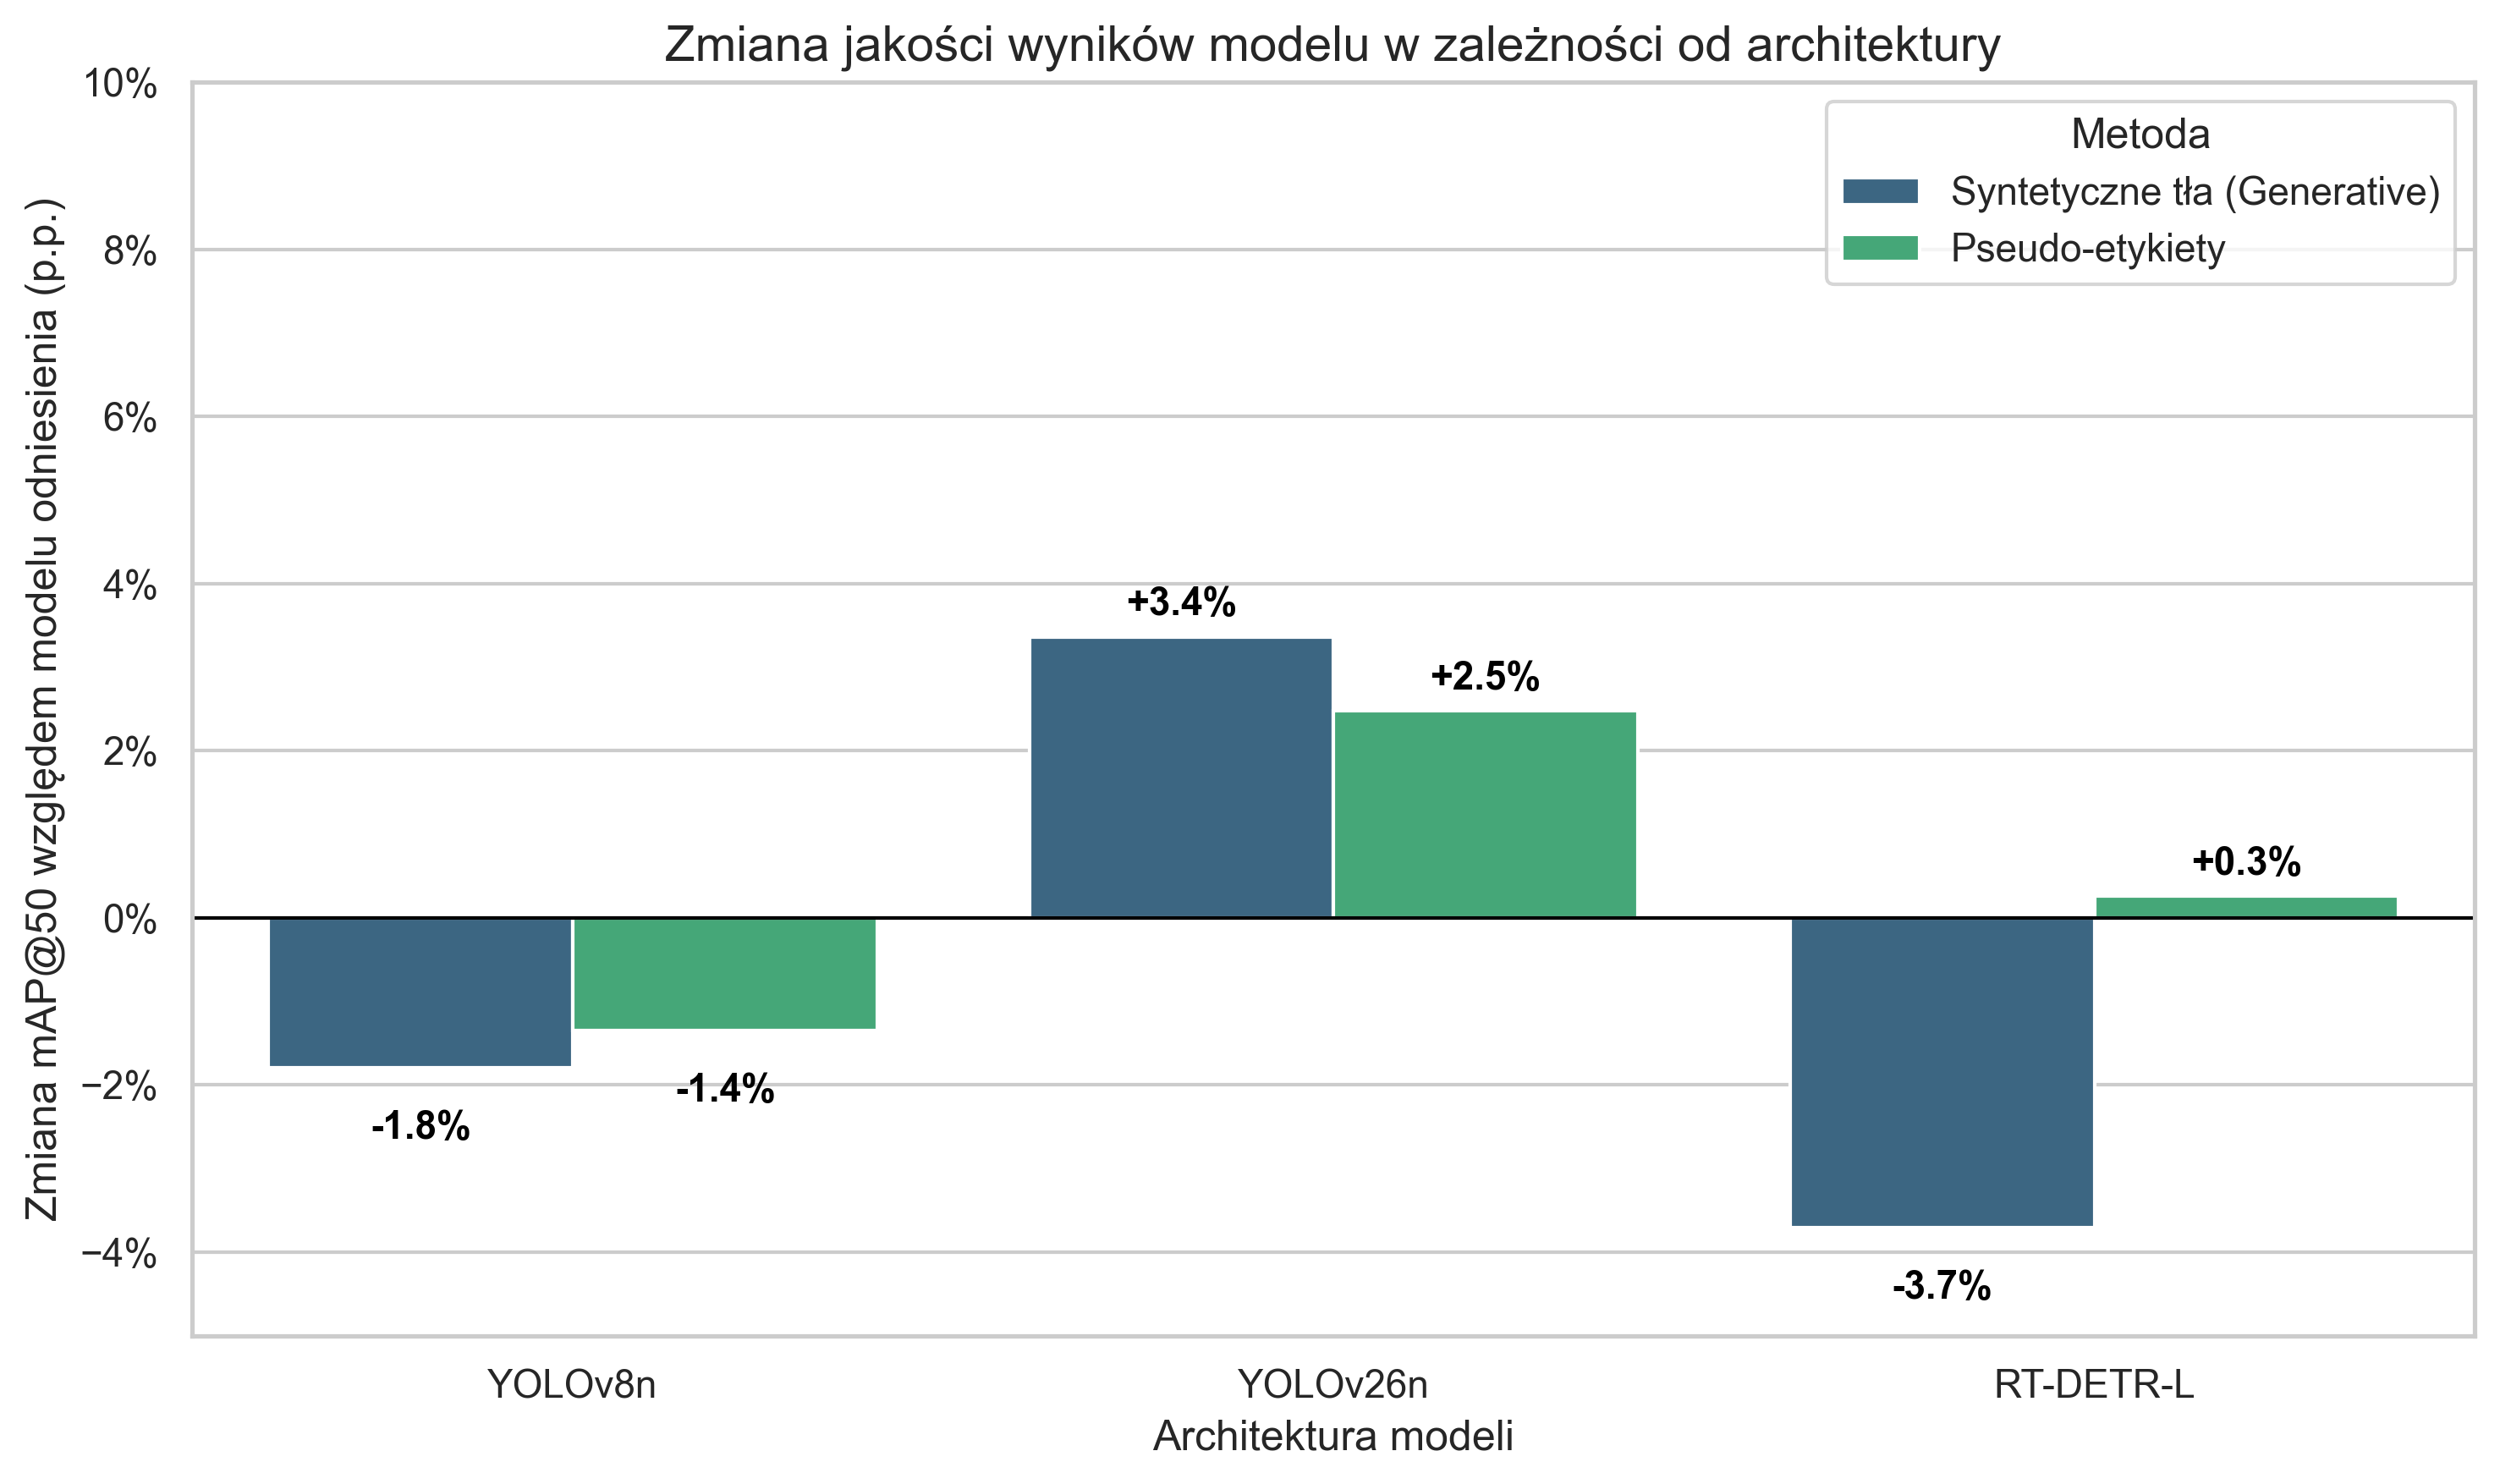
\includegraphics[width=1\linewidth]{Pics/Charts/wykres_3_architektury.png}
\caption{Zmiana jakości wyników modeli w~zależności od architektury oraz zastosowanej metody względem modelu odniesienia.}
\label{fig:susceptibility}
\end{figure}

\begin{enumerate}
\item \textbf{YOLOv8n (model o~wysokim wyniku referencyjnym):} Architektura ta już w~modelu odniesienia osiągnęła wysoką wartość mAP@0.5. Obie formy iteracyjnego SSL obniżyły globalne metryki, choć w~analizie fałszywych detekcji widoczna była częściowa redukcja nadmiarowych wskazań. Wyniki sugerują, że dodatkowe dane nie poprawiły ogólnej jakości lokalizacji, ale mogły ograniczyć skłonność modelu do detekcji w~obszarach tła.

\item \textbf{YOLOv26n (największa poprawa po SSL):} Model ten zanotował wzrosty metryk po zastosowaniu obu wariantów potoku SSL. Wariant z~syntetycznym tłem (+5.1 p.p. mAP@0.5) sprawdził się lepiej niż klasyczne pseudoetykiety (+3.4 p.p. mAP@0.5), co wskazuje, że w~tej architekturze dodatkowe próbki negatywne mogły wspierać rozróżnianie obiektów docelowych od tła.

\item \textbf{RT-DETR-L (wrażliwość na przesunięcie domenowe):} Model ten zachowywał się inaczej niż detektory YOLO. Standardowy proces SSL (Metoda A) nieznacznie poprawił mAP@0.5 oraz F1-score, natomiast dodanie syntetycznych próbek negatywnych (Metoda B) pogorszyło wyniki. Wskazuje to, że architektura oparta na transformerach może być bardziej wrażliwa na artefakty lub przesunięcie domenowe obecne w~danych generowanych syntetycznie.
\end{enumerate}

Osiągnięte rezultaty wskazują, że nie istnieje jedna metoda wzbogacania danych, która w~analizowanym scenariuszu poprawiałaby wyniki wszystkich detektorów. Skuteczność danych nieoznakowanych oraz generowanych syntetycznie zależała od architektury modelu, jakości pseudoetykiet oraz stopnia zgodności danych dodatkowych z~domeną obrazów rzeczywistych. Metody A~i~B analizowano osobno, ponieważ celem pracy było rozdzielenie wpływu pseudoetykietowania od wpływu syntetycznych próbek negatywnych. Połączenie obu metod stanowi naturalny kierunek dalszych eksperymentów, ale jego interpretacja wymagałaby dodatkowej kontroli udziału danych rzeczywistych i~syntetycznych w~zbiorze treningowym.
